%% ****** Start of file apsguide4-2.tex ****** %
%%
%%   This file is part of the APS files in the REVTeX 4.2 distribution.
%%   Version 4.2b of REVTeX, December 2018.
%%
%%   Copyright (c) 2019 The American Physical Society.
%%
%%   See the REVTeX 4.2 README file for restrictions and more information.
%%
\documentclass[twocolumn,secnumarabic,amssymb, nobibnotes, aps, prd]{revtex4-2}
\usepackage{graphicx}
\usepackage{subfigure}
%\usepackage{acrofont}%NOTE: Comment out this line for the release version!
\newcommand{\revtex}{REV\TeX\ }
\newcommand{\classoption}[1]{\texttt{#1}}
\newcommand{\macro}[1]{\texttt{\textbackslash#1}}
\newcommand{\m}[1]{\macro{#1}}
\newcommand{\env}[1]{\texttt{#1}}
\setlength{\textheight}{9.5in}

\begin{document}

\title{Classroom learning dynamics using a cellular automata spatiotemporal model comparing peer instruction and traditional instruction}%

\author{Clarence Ioakim T. Sy}%
\email[Corresponding author: ]{ctsy@up.edu.ph}
\affiliation{National Institute of Physics, University of the Philippines Diliman, Quezon City, Philippines}%
\date{June 2025}%

\begin{abstract}
    Peer instruction (PI) has recently become one of the popular means of classroom instruction in Physics Education. 
    Such instruction method is vastly different from how classes are traditionally handled where the instructor conducts a lecture for the entire duration of the class.
    In this study, we model the transfer of knowledge within the class as a probabilistic cellular automata model and investigate the effects of different factors such as seating arrangements, size, learning rate, and heterogeneity on the classes' overall learning efficiency in peer instruction.
    We compared the learning efficiency between the traditional learning model and the PI model. 
    We found that larger class sizes sway the advantage towards traditional instruction, while increased learning rate heterogeneity favors PI.
    Additionally, an increase in the students' effective learning rate benefits both traditional instruction and PI but in different ways.
    Classes under traditional instruction were found to have two stages of learning when heterogeneity was introduced: a fast initial stage and a slow final stage.
    On the other hand, learning trends in PI were generally unaffected by heterogeneity, having similar effects with the other factors we considered.
    Among the seating arrangements (SAs) we considered for PI, the inner corner SA performed the best in terms of both the time it takes for all the students to learn and the classroom’s learning rate.
    This result differs from previous studies where they found that the outer corner SA performed the best.
    The difference stems from the simplifications made in this model.
    We did not consider the orientation factor of each student, resulting in an isotropic system.
    Our model also uses binary values and does not consider the effect of aptitude similarity that have been described in previous studies. 
    Despite these simplifications, our findings generally agree with previous studies and existing practices that PI performs similarly or better than traditional instruction and that a mix of traditional instruction and PI would be the optimal method of instruction.
    We offer insights based on the qualitative results of the model.
\end{abstract}

\maketitle
\tableofcontents

\section{Peer Instruction and Traditional Models of Instruction}

    Literature discussing peer instruction, especially for physics often cites Mazur's work \textit{Peer Instruction: A User's Manual} \cite{mazur1997peer,mazur1999}.
    In this book, Mazur recounts how he observed a disconnect between students' ability to answer quantitative and conceptual questions in physics.
    He concluded that this resulted from the students' approach of memorizing problem solving algorithms, even if they might not always apply to a given problem.
    Peer Instruction (PI) as a method of instruction aims to address this issue.
    PI forces students to think for themselves and engage with the learning material instead of simply absorbing the information from lectures given by the instructor.
    Engaging with the material allows students to develop a deeper understanding of the concepts and apply them to different problems.
    This has been shown to not only apply in high school physics, but also in other disciplines and higher education \cite{johnson2008active,fagen2000factors,fagen2002peer}.

    \subsection{Difference of Peer Instruction from Traditional Instruction}

    There are many ways to implement PI in the classroom.
    The method outlined by Mazur \cite{mazur1997peer} involves the instructor giving a short lecture on a topic, followed by a multiple choice question (MCQ) that the students answer individually.
    The students then discuss their answers with their peers before answering an MCQ again.
    Variations can be made depending on the class set up and the instructor.
    
    This is in stark contrast with how traditional instruction (TI) is conducted where the instructor often just gives a lecture for the entire duration of the class.
    PI is meant to be student centric, meaning that the instructor is expected to make differences to the steps outlined above to adjust to the class's needs.
    The MCQs can be graded or ungraded \cite{crouch2001peer}, the instructor can choose to give multiple MCQs and peer discussion opportunities during one class, or the instructor can choose to give a different MCQ after the discussion as long as it still tackles the same learning objective \cite{smith2009peer}.
    If only a few students answer the MCQ correctly, the instructor can even give a short lecture to clarify the concept \cite{lasry2008peer}.

    \subsection{Benefits of PI}

    Despite the de-emphasis on problem-solving in PI lectures, students' quantitative problem-solving skills were not compromised and was even improved compared to traditional instruction in some cases.
    PI was also find to significantly decrease the number of of students with extremely low scores \cite{crouch2001peer}.
    This is consistent with findings of other studies \cite{lasry2008peer,thacker1994comparing}.
    Similarly, students' conceptual understanding of the lessons also improved.
    This holds true for both in-class concept tests and end-of-semester exams \cite{crouch2001peer}.

    Smith, et. al \cite{smith2009peer} modified the PI method to make sure that students were not copying off of each other. After the first MCQ, he did not show the class's answer statistics and used a pair of isomorphic questions for the MCQs before and after the peer discussion section. Isomorphic questions are questions that tackle the same learning objectives but have different "cover stories".
    They also found that even in groups whose members were not able to answer the first MCQ, students were able to get the correct answer for the second MCQ.
    This contradicts the transmissionist view of PI where students only learn from other students who already know the lesson.
    The study provides evidence that PI can be viewed as constructivist where students learn on their own through discussion and not simply from hearing the correct answer.

    In addition to those mentioned above Lasry, et. al. \cite{lasry2008peer} showed that PI is not necessarily dependent on background knowledge. They found that students in under PI performed as well as or better than those under TI despite the former having less background knowledge.
    They also found the PI greatly reduced the number of students who dropped the course.
    An older paper by Tobias \cite{tobias1990they} suggests that this could be because of the shift of focus of PI from competition and skill performance to cooperative learning and conceptual understanding.


\section{Existing Mathematical Models of PI}

    Although there are some mathematical models for learning, the ones that describe learning in the classroom are few and far in between - even more so for those that model PI.

    Roxas et al. \cite{roxas2010seating} used actual assessment results to train a neural network to map student interactions in PI classrooms. 
    Using this neural network, they were able to characterize information transfer and investigate the effects of group homogeneity. 
    Their study also investigated the optimal seating arrangement for students under PI methods based on their aptitude.
    In their paper, the measure of students' improvement was calculated via the Hake gain as shown in Equation~\ref{eq: hake gain} \cite{hake1998}.
    They also used the output/input ratio (O/I), which was the ratio of second assessment scores vs first assessment scores, to gauge student improvement.
    However, it should be noted that O/I values tend to be biased towards low-scoring students.
    \begin{equation}
        \label{eq: hake gain}
        \langle g \rangle = \frac{\langle 2^{\text{nd}}\text{ assessment} - 1^{\text{st}}\text{ assessment} \rangle}{\langle 1 - 1^{\text{st}}\text{ assessment} \rangle}
    \end{equation}

    The results of their study show that the outer corner seating arrangement (SA) performed the best, followed by inner corner, then random, then center (see Figure~\ref{fig:PI SAs} for SA visualizations).
    In simulated classrooms, each with 64 students and 10 classrooms in total, they found that homogenous classrooms with low aptitudes have significantly higher O/I values.
    This means that low aptitude students benefit the most from being grouped together.

    \begin{figure}[htbp!]
        \centering
        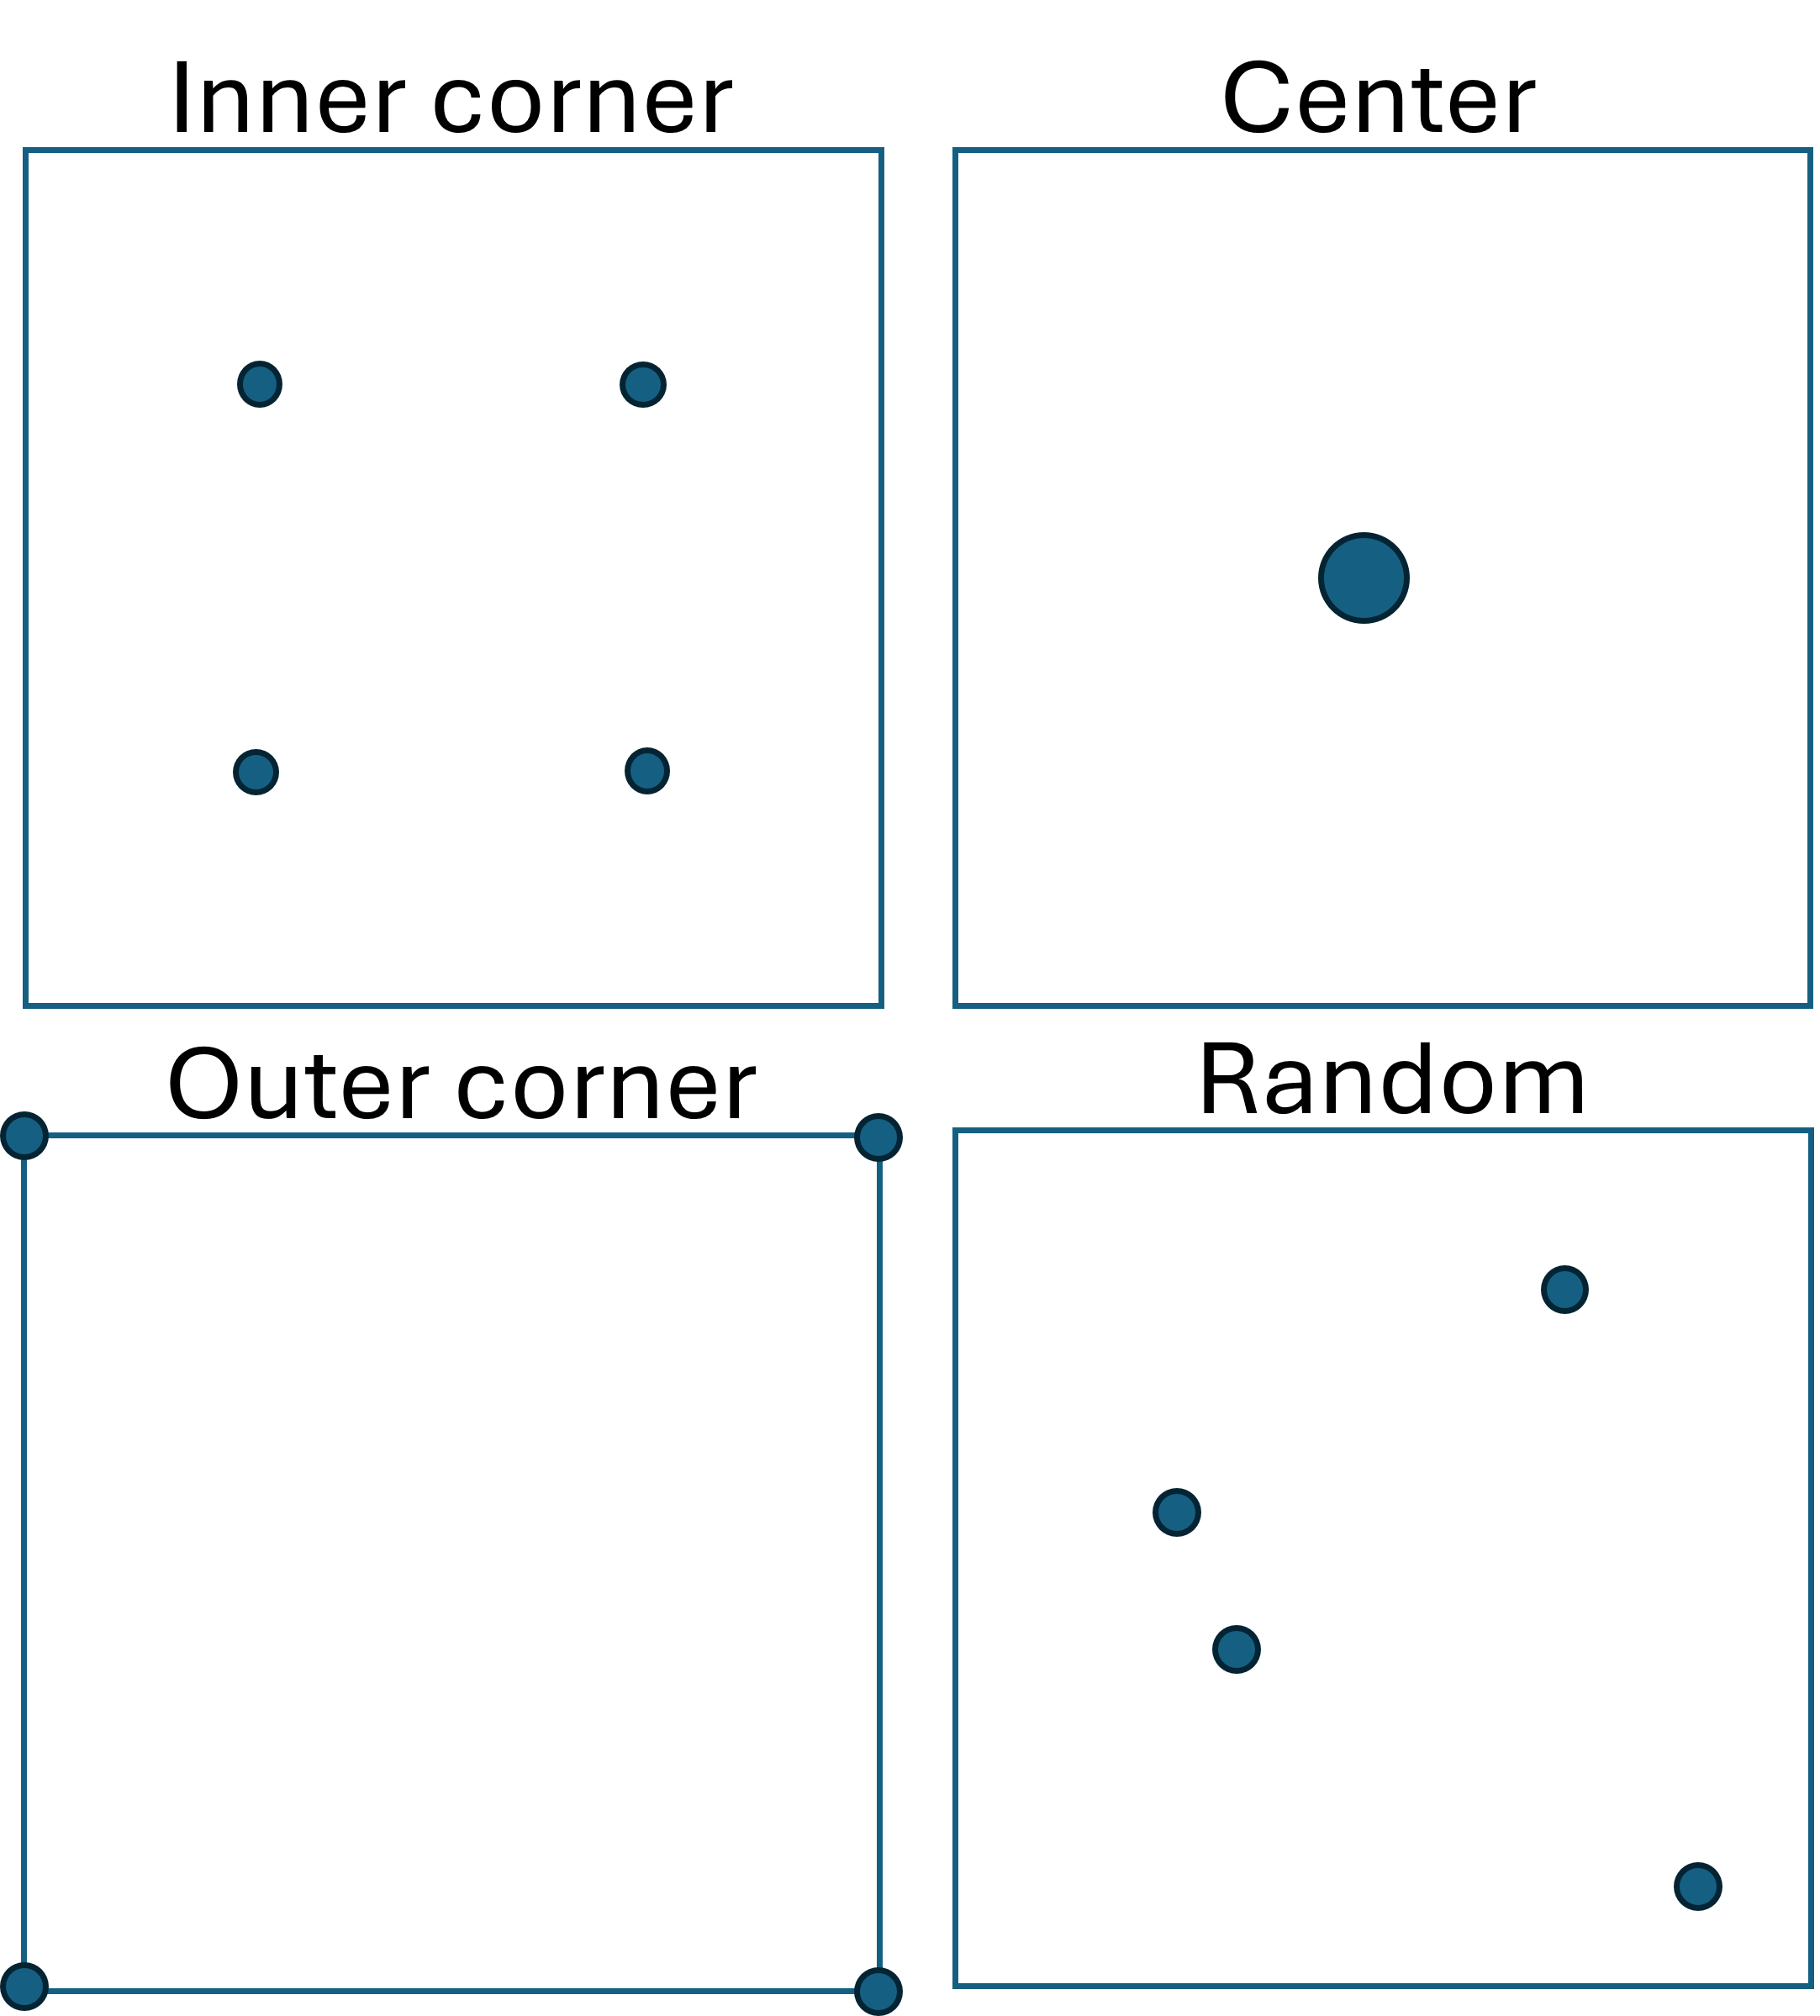
\includegraphics[width=0.40\textwidth]{figures/PI SAs.png}
        \caption{Seating arrangements considered for PI}
        \label{fig:PI SAs}
    \end{figure}

    Nitta \cite{nitta2019mathematical} gives us a few existing models that model PI. 
    One of the models that was presented is a generalized Ising Model by Bordogna and Albano \cite{bordogna2001theoretical,bordogna2003simulation} where they consider three sources of information for the student to learn from: teacher instruction, peer interaction, and bibliographic materials (books, lecture notes, etc.)
    Their model shows that students learn more when they engage discussions with their peers than those who only listen to lectures.
    They also show that group structure affects student learning, and that low aptitude students may learn at the expense of high aptitude peers - a transmissionist view of PI.

    Nitta also presents a model by Pritchard et al \cite{pritchard2008mathematical} where PI is modeled as a set differential equations that is dependent on the probability of students learning to stick (memory model, Equation~\ref{eq:memory model}) and the ability for students to associate new learnings from old knowledge via logistic differential equation (connectedness model, Equation~\ref{eq:connectedness model}.)

    Memory model:
    \begin{equation}
        \label{eq:memory model}
        \frac{dU_T(t)}{dt} = -\alpha_m U_T(t)
    \end{equation}

    Connectedness model:
    \begin{equation}
        \label{eq:connectedness model}
        \frac{dU_T(t)}{dt} = -\alpha_c U_T(t)K_T(t)
    \end{equation}

    where knowledge is taken to grow at a uniform rate, as in the tutoring model:
    \begin{equation}
        \label{eq:tutoring model}
        K_T(t) = \alpha_{tu}t + K_T(0)
    \end{equation}
    \begin{equation}
        U(t) + K(T) = 1
    \end{equation}

    In these equations $U(T)$ and $K(T)$ are the unknown and known knowledge domains respectively. $\alpha_m$, $\alpha_c$, and $\alpha_{tu}$ are the corresponding rates for the memory model, connectedness model, and tutoring model 

    In deriving their own equations to model PI, Nitta arrived at equations similar to Hake gain to evaluate the effectiveness of PI for a concept test question and Pritchard's connectedness model to model the classes' learning processes.
    Comparing their equations to data, they concluded that these metrics and equations roughly agree with the data and could give us insights on the learning dynamics of the classroom.

    The process of PI is complex, with many interacting components.
    Existing models are either predictive, as in the case of the neural network modeling of Roxas et al. \cite{roxas2010seating} or lack the spatial aspect of the process as with the differential equations of Pritchard \cite{pritchard2008mathematical} and Nitta \cite{nitta2019mathematical}.
    While Bordogna et al. \cite{bordogna2001theoretical,bordogna2003simulation} present to us a dynamical model in their generalized Ising model, it lacks some of the aspects of PI we'd like to consider like seating arrangements, students' learning rate, and heterogeneity.

    We propose that a probabilistic cellular automata model can be used to study the spatiotemporal dynamics of both PI and traditional instruction when incorporating these different aspects into the model.
    We previously used a probabilistic cellular automata to model the classroom \cite{SelfSPP}, the results of which were presented in the 42$^{\text{nd}}$ Samahang Pisika ng Pilipinas Conference in July 2024.
    The findings presented in the paper are also presented in this study as part of the results.

\section{Modelling The Classroom As A Probabilistic Cellular Automaton}

    We use a probabilistic cellular automata (PCA) model to simulate the learning process in the classroom.
    In this PCA model, each cell in the automaton represents a student where each student is assigned a learning rate $\lambda_{i,j}$ to describe how fast they learn as an individual.
    The state of each cell represents their aptitude $s_{i,j}=\lbrace\text{unlearned},\text{learned}\rbrace=\lbrace0,1\rbrace$.
    We assign the neighborhood to be an outer totalistic Moore neighborhood of radius $r=1$ and define the boundary conditions to be fixed wherein the grid does not wrap around itself and $s_{i,j}=0 \text{ for }i,j\notin[1,L]$.
    For each time step, we find the probability of a student to learn and update the state of the student based on this probability.
    The probability of a student to learn is calculated differently for traditional instruction and peer instruction.

    \subsection{Update Rules for Traditional Instruction (TI)}

        For traditional instruction, the probability of a student to learn in each time step ($P_{i,j}$) is given by:

        \begin{equation}
            P_{i,j} = \lambda_{i,j}\rho_0
        \end{equation}

        where

        $P_{i,j} \in [0,1]$ is the probability of student $c_{i,j}$ to learn in each time step, 

        $\lambda_{i,j} \in [0,1]$ is the learning rate of student $c_{i,j}$

        $\rho_{0} \in [0,1]$ is the probability of $c_{i,j}$ to learn from the teacher based on their relative position from the teacher.

        We consider the case that students have heterogeneous learning rates $\lambda_{i,j}=\lambda_0 \pm \delta\lambda$ where $\lambda_0=0.5$.
        This allows us to investigate the effects of student heterogeneity on the classroom's learning dynamics.

        Having a positional learning coefficient $\rho_{i,j}$ allows us to model a classroom where students closer to the teacher in front learn faster than those farther away or vice versa.
        However, for this research, we only consider the case such that $\rho_{i,j} = \rho_0 \forall i,j$.

        The numerical procedure is outlined in Figure~\ref{fig:TI flowchart}.
        Each simulation for the TI model starts with all students unlearned.
        The simulation is considered finished once all the students have learned.

        \begin{figure}[htbp!]
            \centering
            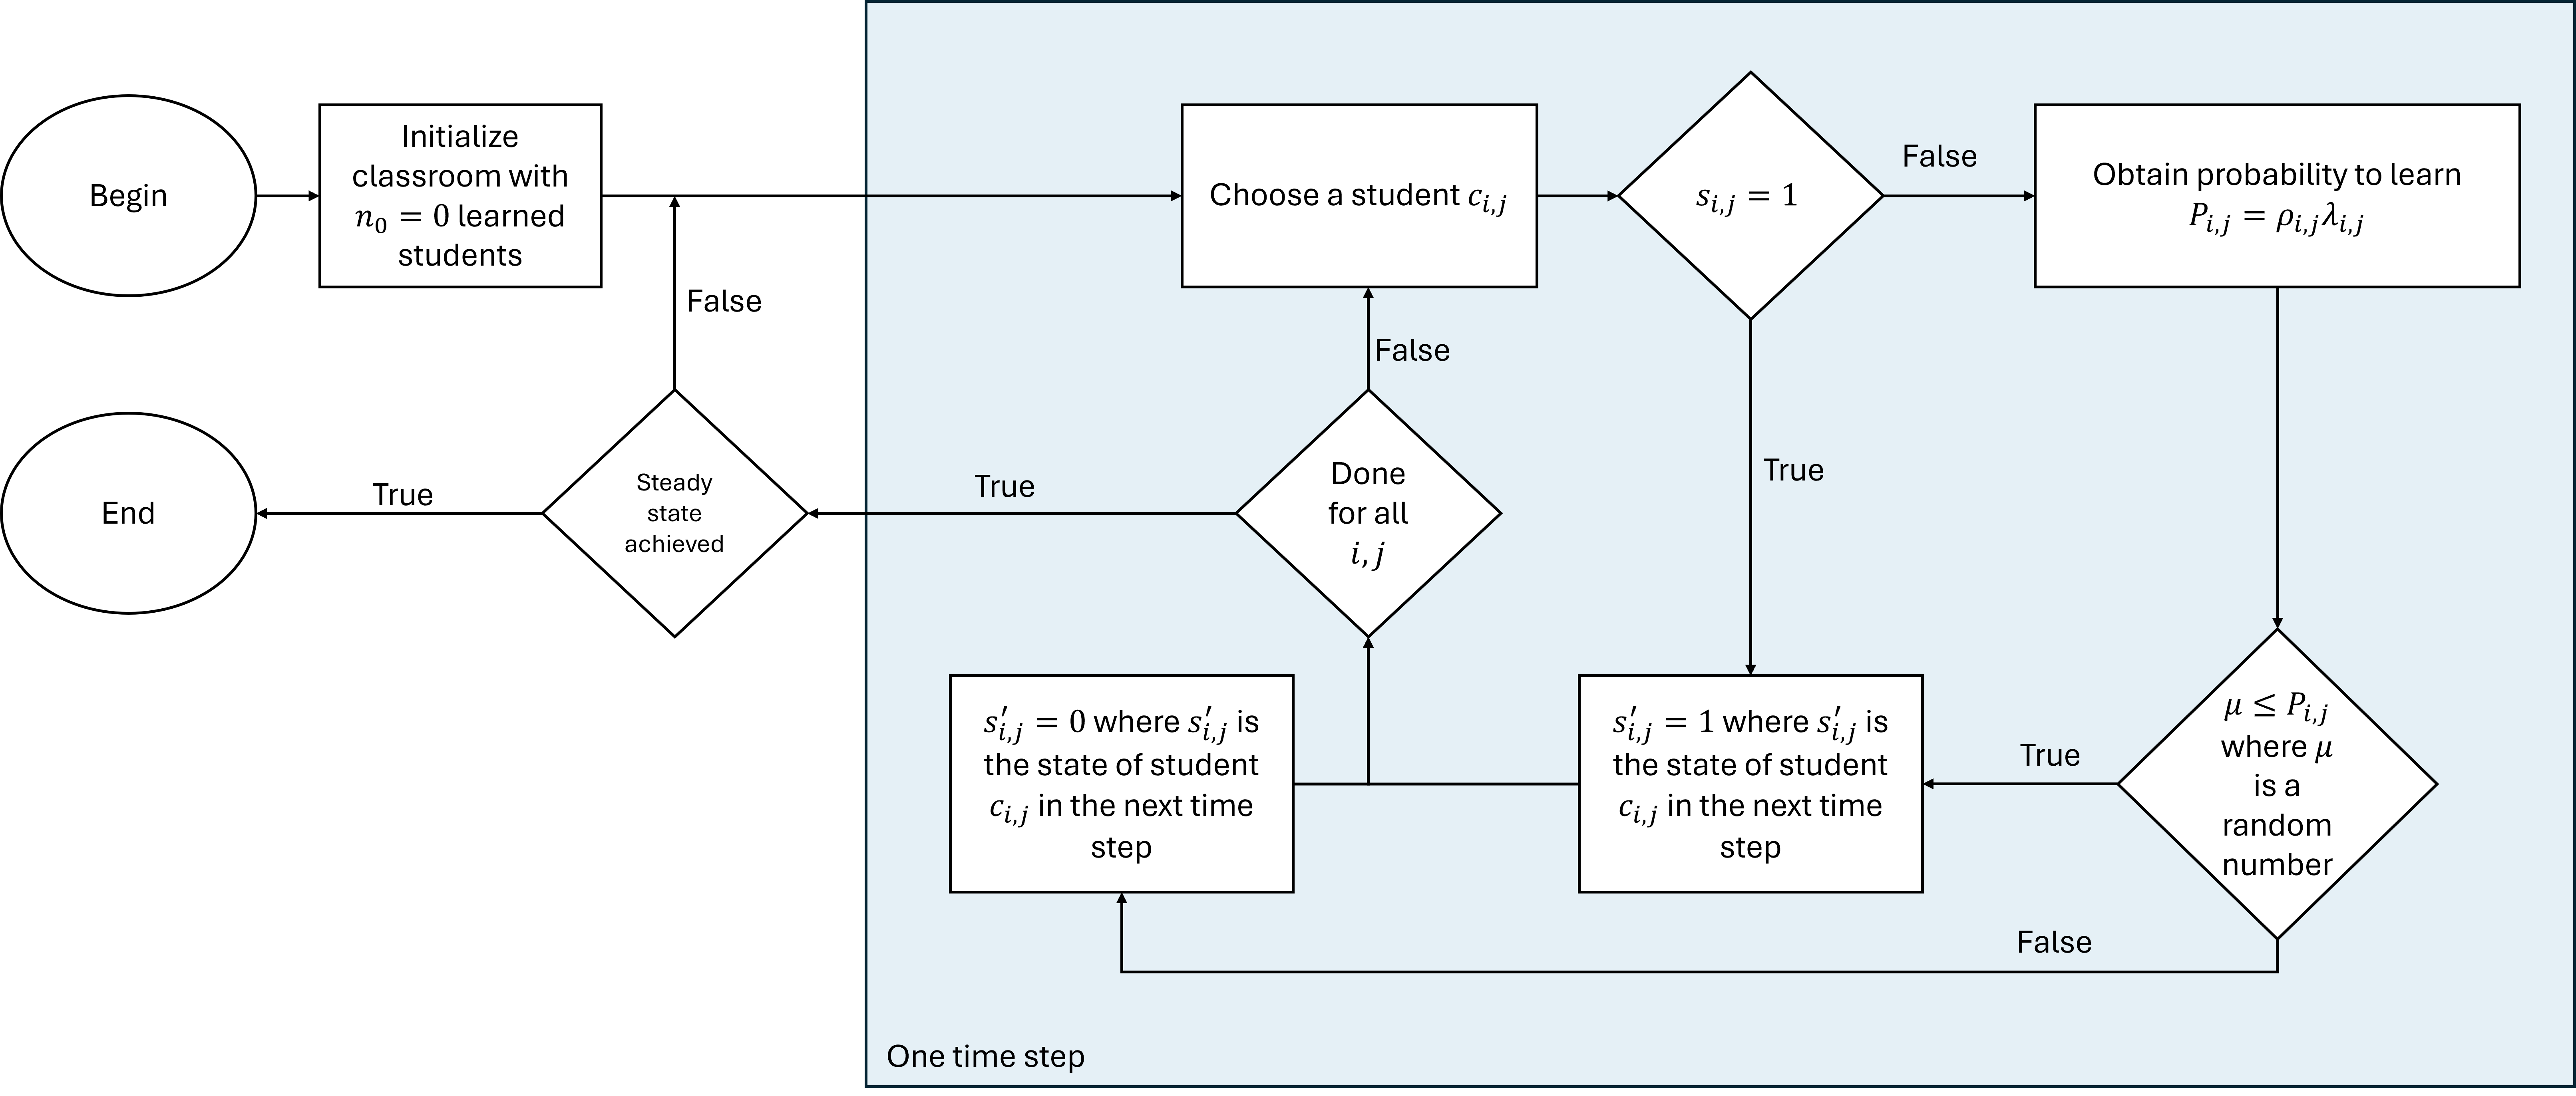
\includegraphics[width=0.45\textwidth]{figures/2DBPCA TI Flowchart.png}
            \caption[Traditional instruction simulation flowchart]{Numerical process for simulation of 2D BPCA for traditional setups.}
            \label{fig:TI flowchart}
        \end{figure}

    \subsection{Update Rules for Peer Instruction (PI)}

        In contrast to TI, the probability of a student to learn in each time step for PI is additionally dependent on the student's neighbors and their states. The probability of a student to learn in each time step ($P_{i,j}$) is given by:

        \begin{equation}
            \label{eq:BPCA PI learning probability}
                P_{i,j} = 1 - \prod_{\forall \delta i, \delta j}{\lbrack1-(\lambda_{i,j})(\rho_{\delta i, \delta j})(s_{i+\delta i, j+\delta j})}\rbrack
        \end{equation}
        
        where
        
        $P_{i,j} \in [0,1]$ is the probability of student $c_{i,j}$ to learn in each time step, 
        
        $\lambda_{i,j} \in  [0,1]$ is the learning rate of student $c_{i,j}$. We consider the case that students have heterogeneous learning rates $\lambda_{i,j}=\lambda_0 \pm \delta\lambda$ where $\lambda_0=0.5$.
        
        $\rho_{\delta i, \delta j} \in [0,1]$ is the probability of $c_{i,j}$ to learn from their neighbors in seats $\lbrace c_{i+\delta i, j+\delta j} \forall \delta i, \delta j \in \lbrace -1,0,1 \rbrace \rbrace$ solely based from their relative positions with each other, and
        
        $s_{i+\delta i, j+\delta j} = \lbrace\text{unlearned, learned}\rbrace=\lbrace 0,1 \rbrace$ are the neighbors' aptitude level.

        The numerical procedure is outlined in Figure~\ref{fig:PI flowchart}.
        Each simulation for the PI model starts with only four learned students $n_0 = 4$.
        The simulation is considered finished once all the students have learned.

        \begin{figure}[htbp!]
            \centering
            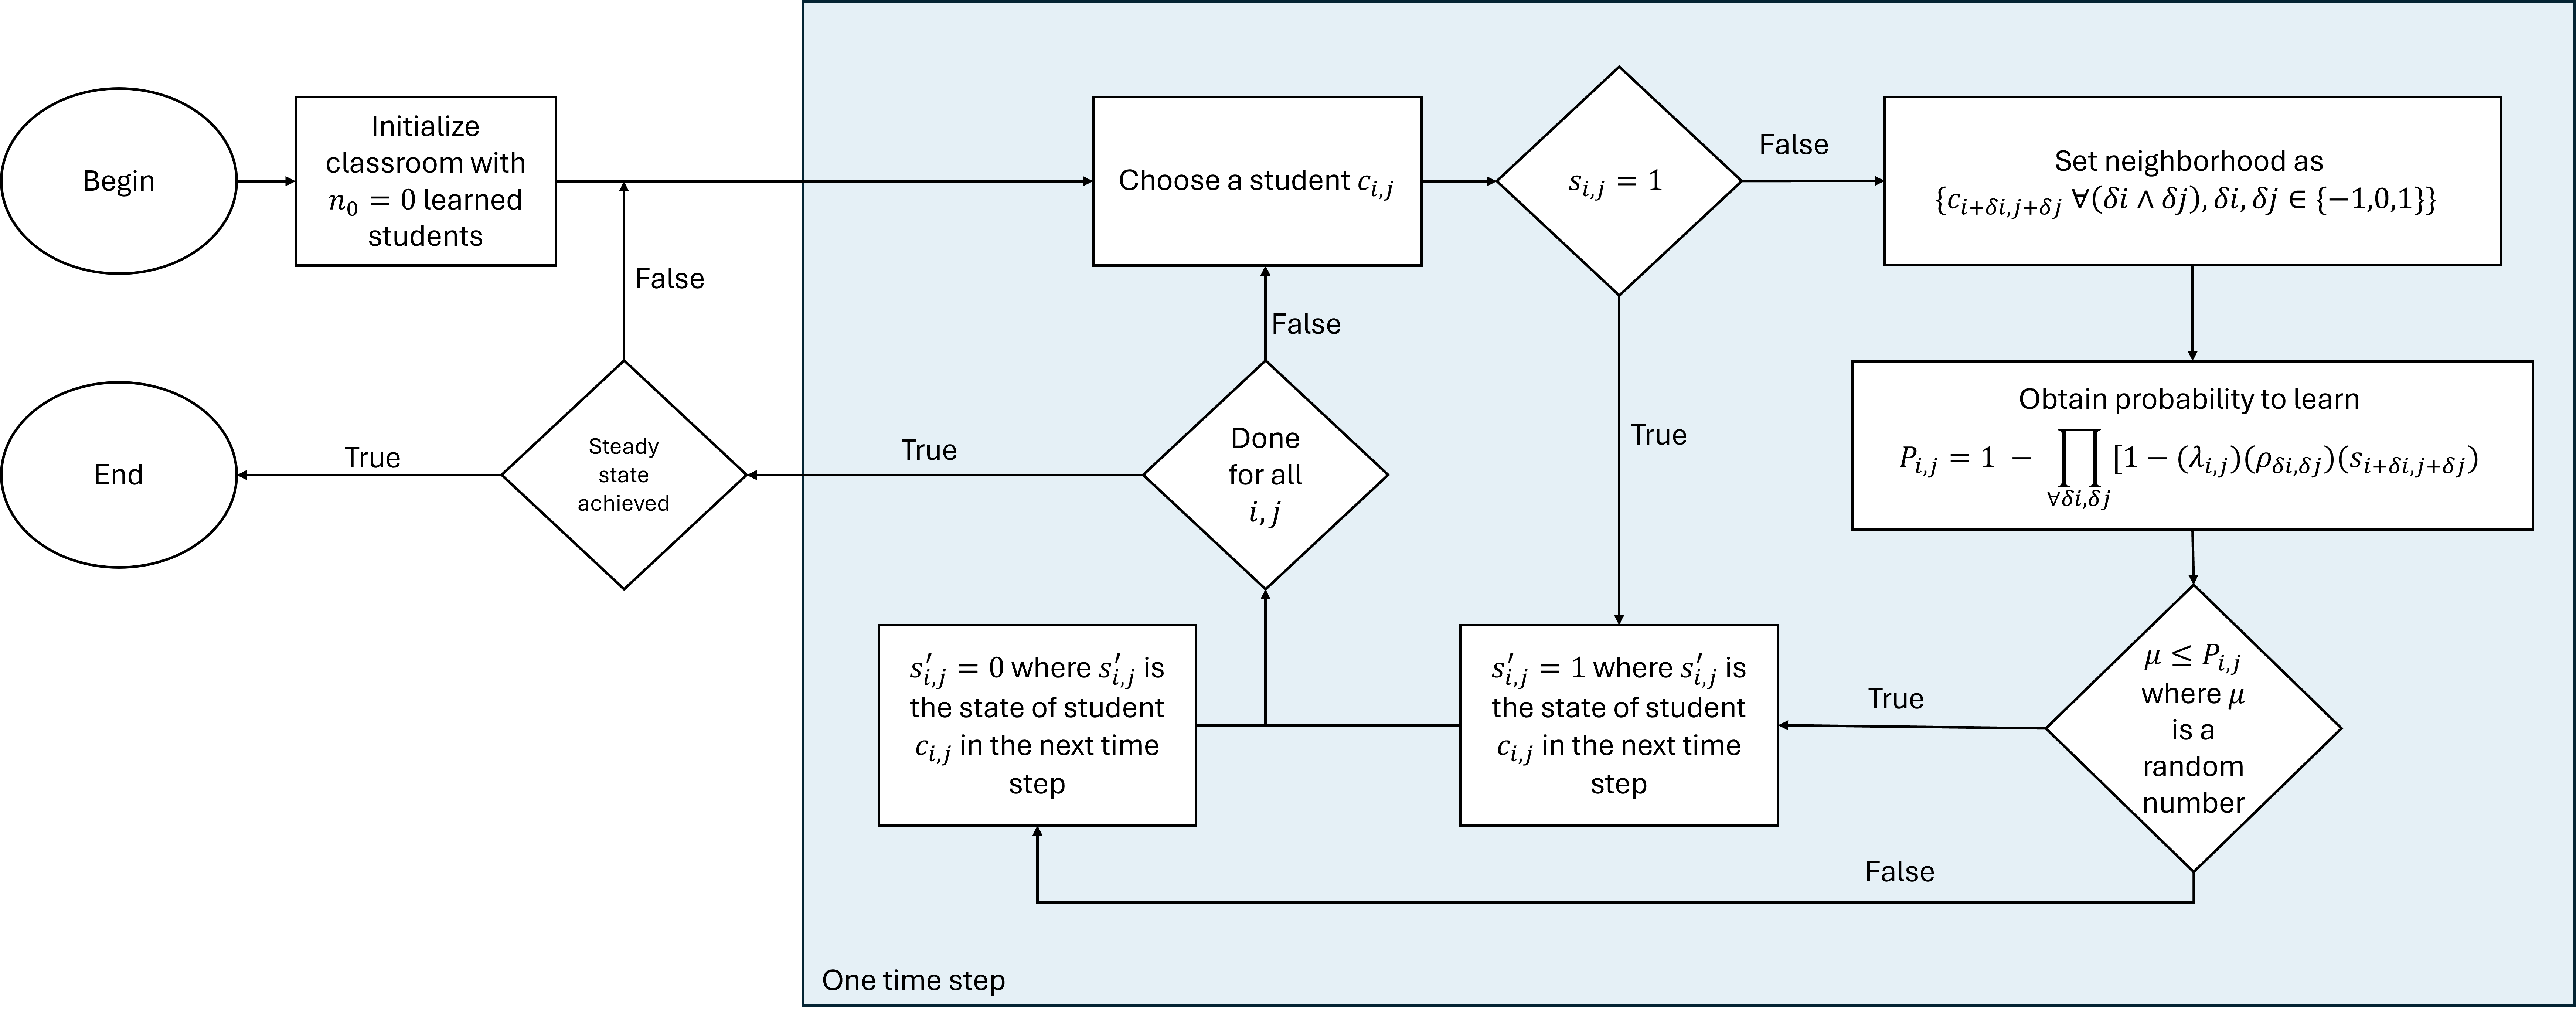
\includegraphics[width=0.45\textwidth]{figures/2DBPCA PI Flowchart.png}
            \caption[Peer instruction simulation flowchart]{Numerical process for simulation of 2D BPCA for PI setups.}
            \label{fig:PI flowchart}
        \end{figure}


    \subsection{Model parameters}
        The values of the model input parameters we considered for the class size $L$, the positional learning coefficient $\rho_0$, and the learning rate heterogeneity $\delta\lambda$ are as follows:

        \begin{itemize}
            \item $L=\lbrace32,48,64,96,128\rbrace$
            \item $\rho_0=\lbrace0.1, 0.2, 0.3,\dots, 0.8, 0.9, 1.0\rbrace$
            \item $\delta\lambda=\lbrace0.0, 0.1, 0.2, 0.3, 0.4\rbrace$
        \end{itemize}

        To assess how well the class learned, we used to parameters --- the time it took for all the students to learn $t_{max}$ and the class's average learning rate $m$.
        The time it took for all the students to learn $t_{max}$ was calculated as the number of time steps it took for all the students to learn.
        The class's average learning rate $m$ was calculated by taking the fraction of learned students as a function of time then fitting a power law ($y=ax^m$) to a fraction of the data using the Levenberg-Marquardt algorithm.
        We chose to fit the power law only to the first half or quarter of the data for peer instruction and traditional instruction respectively so that we obtain the class learning rate before the finite size effect become significant.

\section{Results and Discussion}
    % Discussion outline:
    % \begin{itemize}
    %     \item Results $\rightarrow$ plots $\rightarrow$ interpretation
    %     \item Comparison with existing research
    % \end{itemize}

    % Lorem ipsum dolor sit amet, consectetur adipisci elit, sed eiusmod tempor incidunt ut labore et dolore magna aliqua. Ut enim ad minim veniam, quis nostrum exercitationem ullam corporis suscipit laboriosam, nisi ut aliquid ex ea commodi consequatur. Quis aute iure reprehenderit in voluptate velit esse cillum dolore eu fugiat nulla pariatur. Excepteur sint obcaecat cupiditat non proident, sunt in culpa qui officia deserunt mollit anim id est laborum

    \subsection{Different Dynamics of Traditional and Peer Instruction}
        
        When we vary class size $N$, as shown in Figure~\ref{fig:comparison size}, we see that in TI remains constant with only time to learn $t_{max}$ increasing with class size $N$.
        For PI, increasing class size $N$ adds a time delay to when the learning starts to speed up. Despite the added time delay, the shape of the learning curve remains the same.
        The increase in time to learn $t_{max}$ is also less pronounced in PI compared to TI.

        \begin{figure}[htbp!]
            \centering
            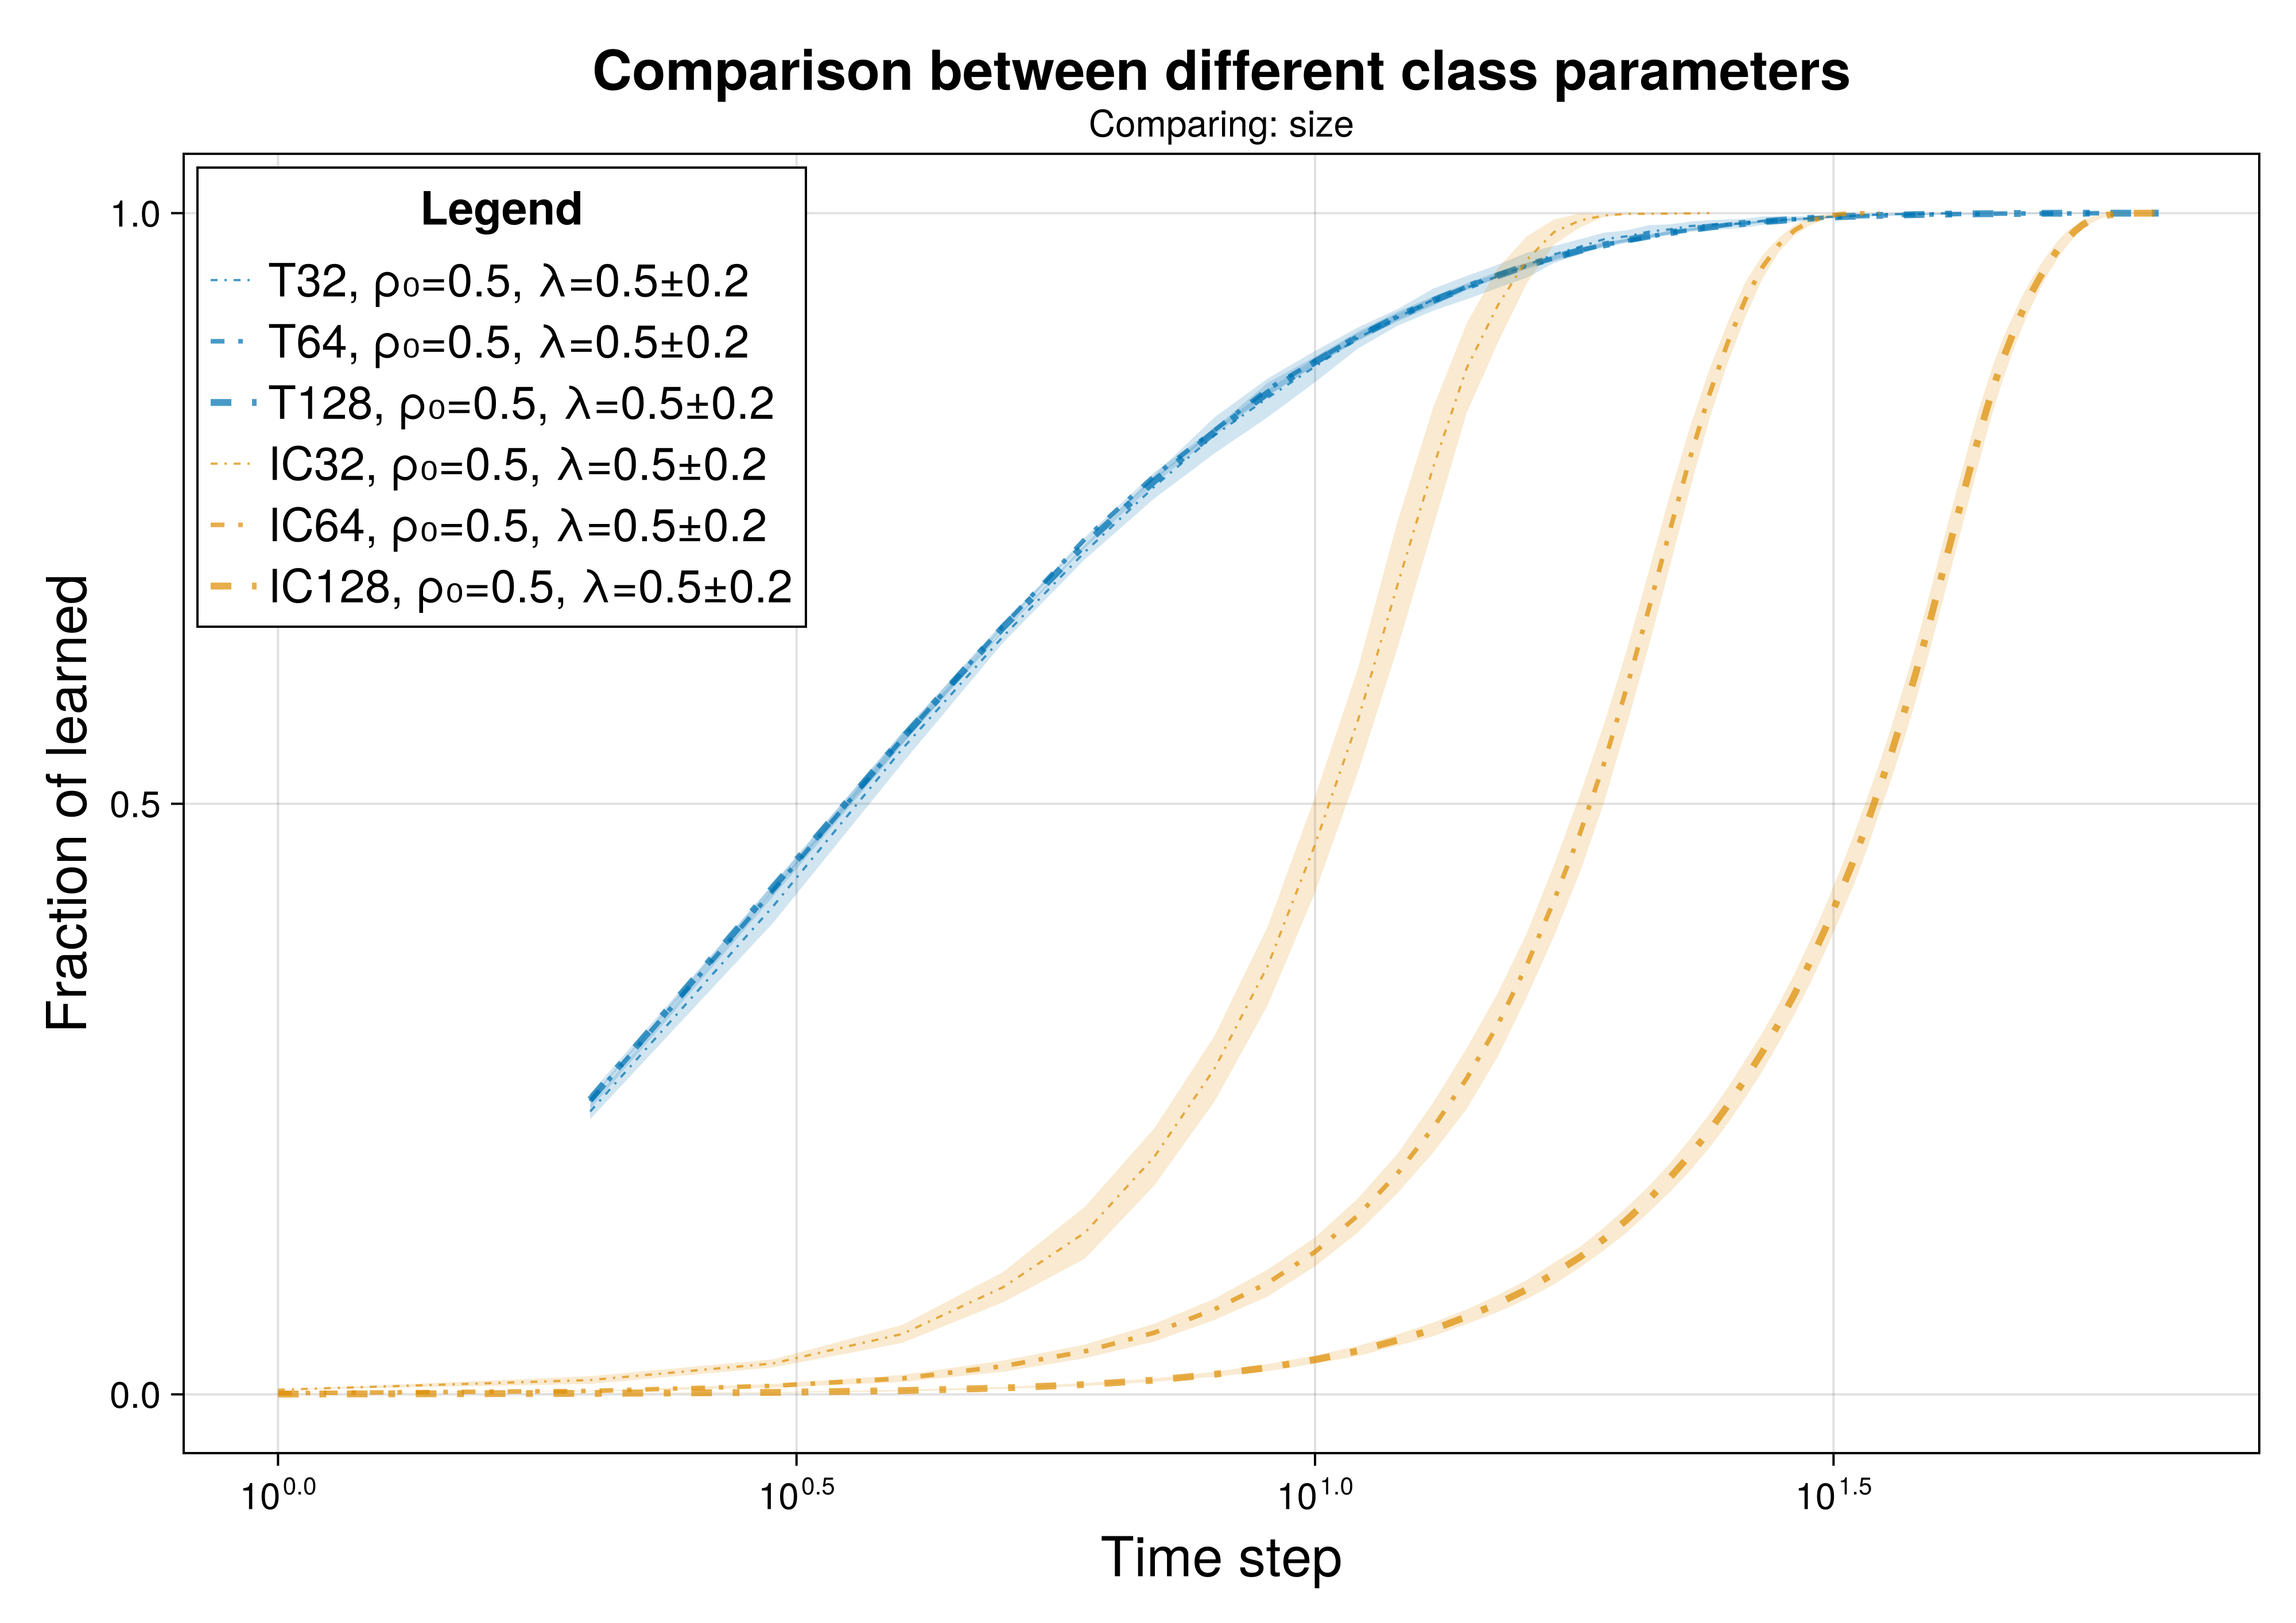
\includegraphics[width=0.45\textwidth]{figures/2D-BPCAIH-analysis/comparison plots/size.png}
            \caption{Comparison of learning dynamics for different class sizes $N$}
            \label{fig:comparison size}
        \end{figure}

        Varying positional learning factor $\rho_0$, shown in Figure~\ref{fig:comparison ρ₀}, varies the shape of the learning curve for TI, especially for lower values of positional learning factor $\rho_0$.
        For traditional instruction, changes in $\rho_0$ affects the number of students that learn in the second time step and the rate of which students learn throughout the class.
        For peer instruction, the shape of the learning curve remains the same for different values of $\rho_0$, only adding a time delay to when the learning starts to speed up --- similar to the effects of class size $N$.
        Additionally, the effect of varying positional learning factor $\rho_0$ is nonlinear for both models. Those with extremely low values of $\rho_0$, like those of $\rho_0=0.1$, perform much worse with learning curves being further from $\rho_0=0.5$ than $\rho_0=0.9$ is with $\rho_0=0.5$.

        \begin{figure}[htbp!]
            \centering
            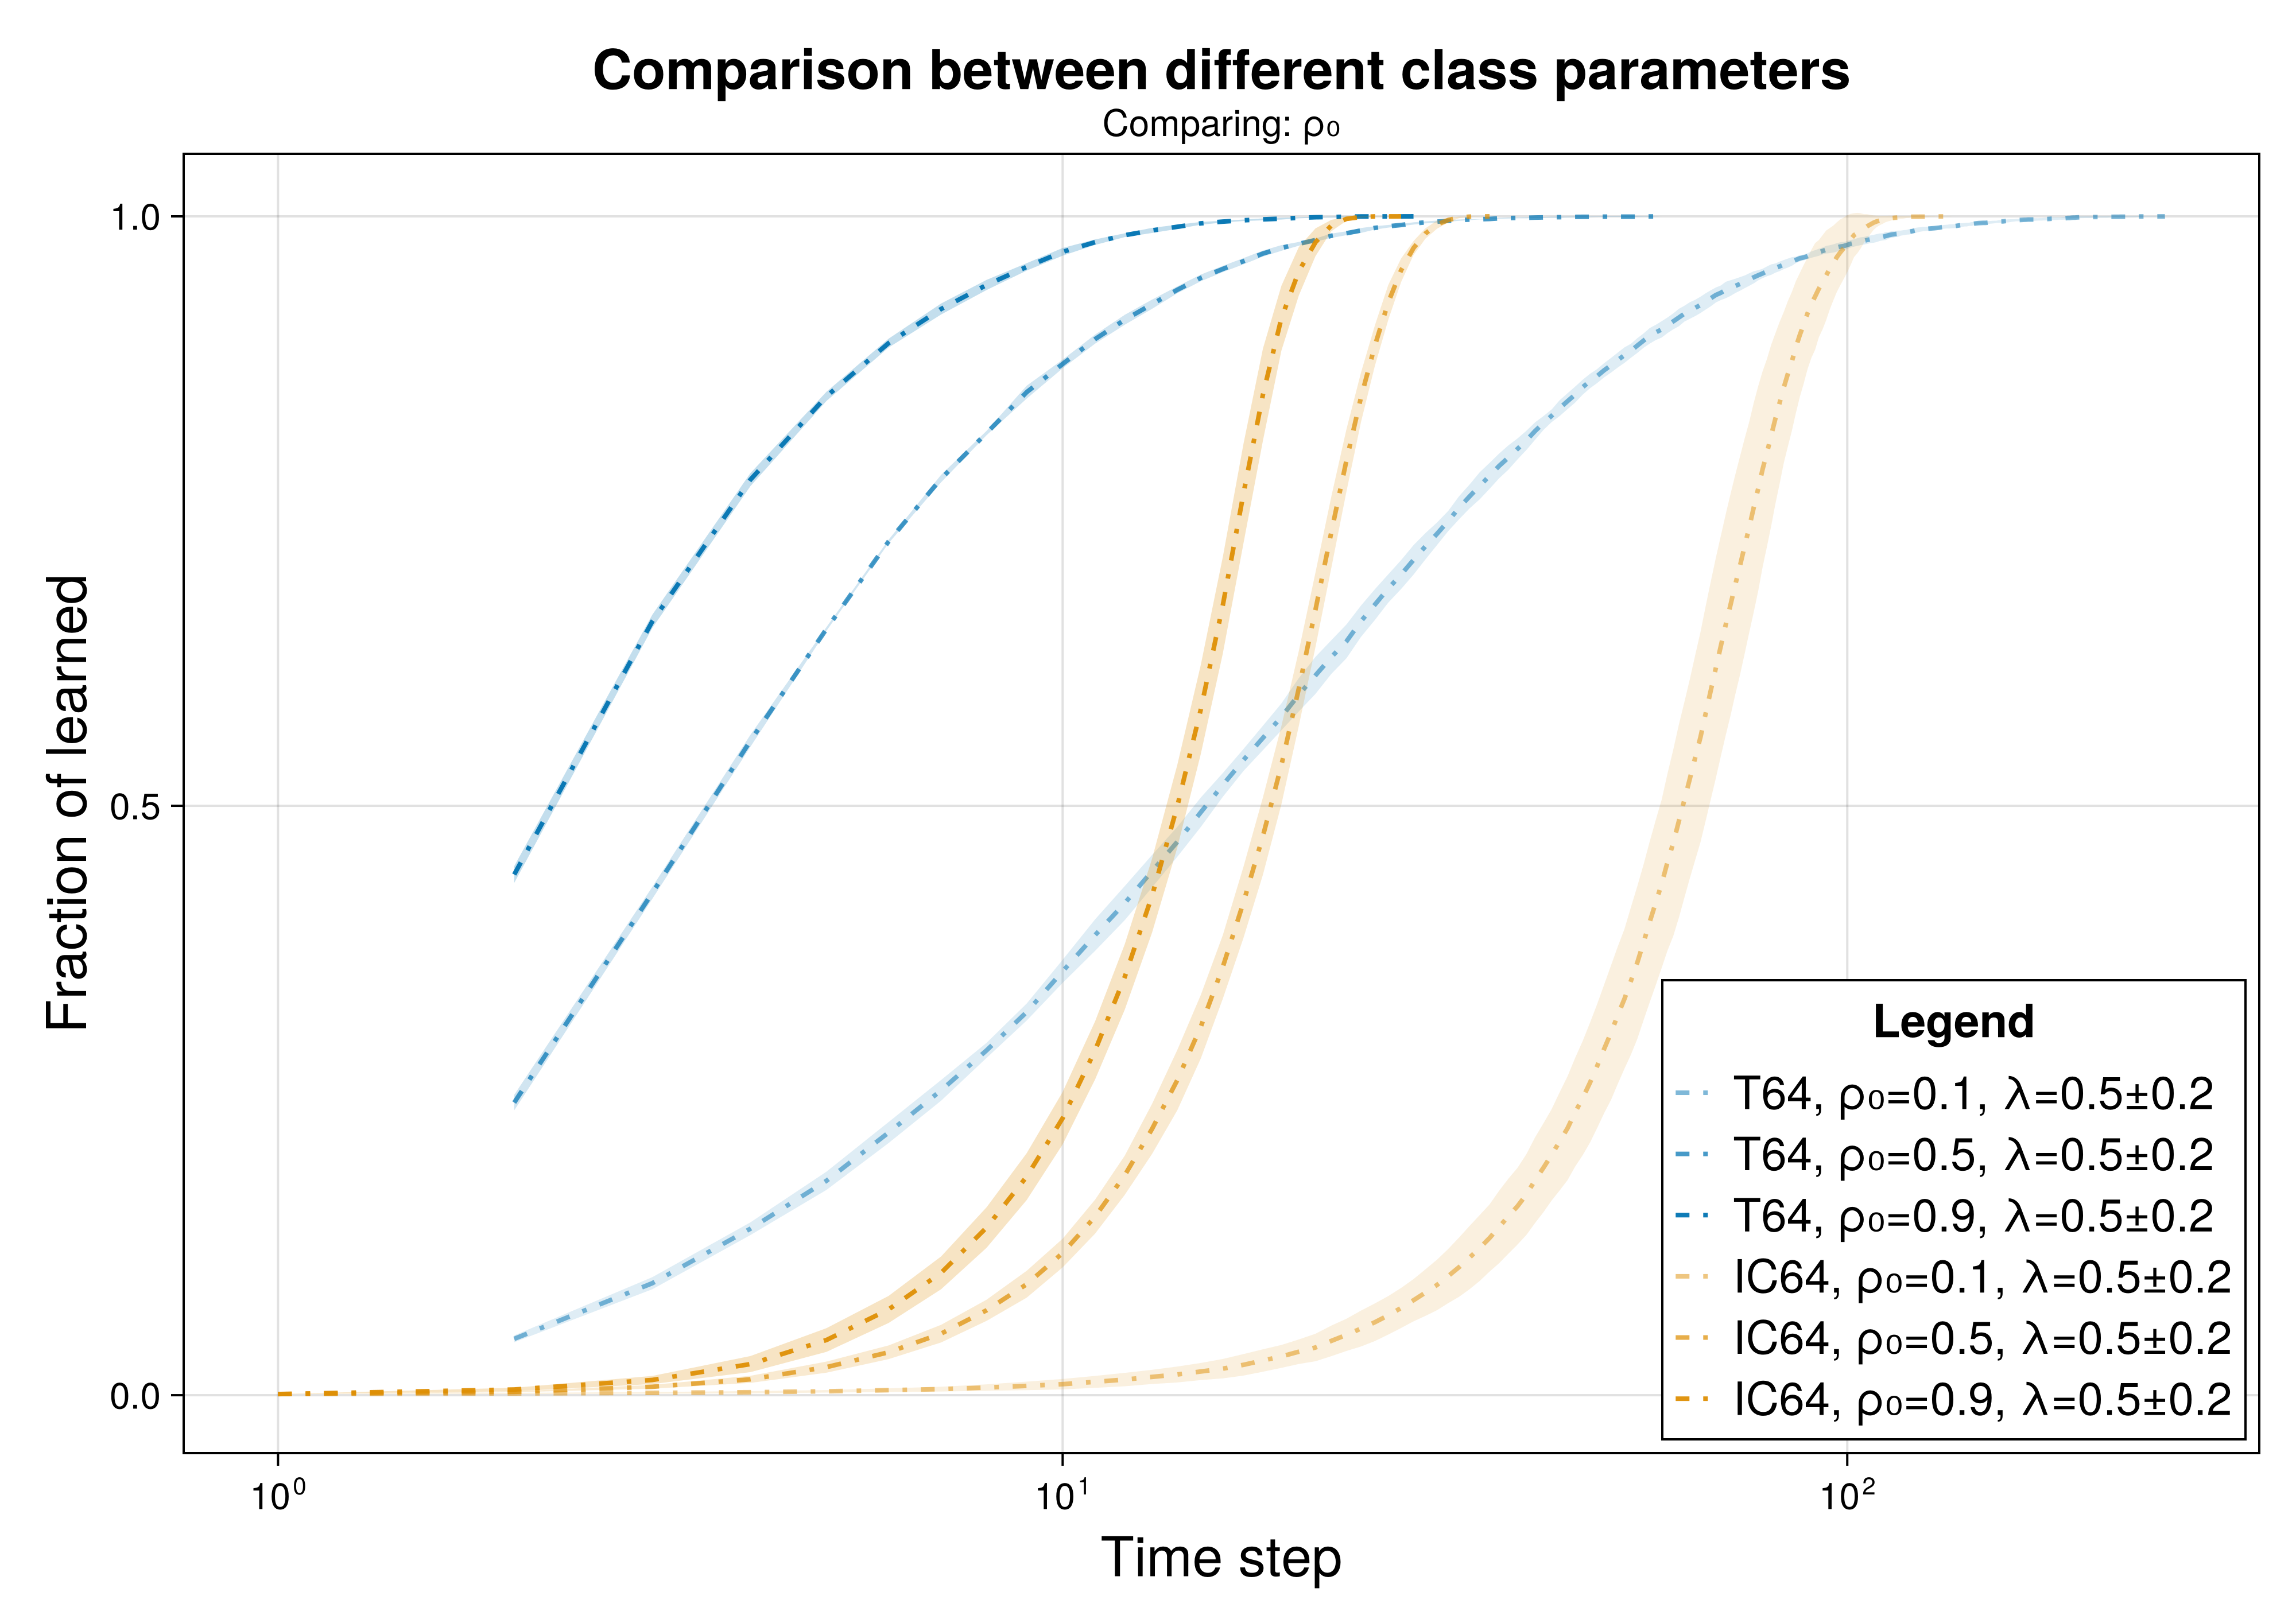
\includegraphics[width=0.45\textwidth]{figures/2D-BPCAIH-analysis/comparison plots/ρ₀.png}
            \caption{Comparison of learning dynamics for different positional learning factor $\rho_0$}
            \label{fig:comparison ρ₀}
        \end{figure}

        Figure~\ref{fig:comparison δλ} shows that an increase in heterogeneity $\delta\lambda$ changes how fast the slope of the learning curve changes for TI without changing the initial number of learned students.
        For PI, only very high values of heterogeneity $\delta\lambda$ noticeably affect the learning curve.
        As with the positional learning factor $\rho_0$, the effect of varying heterogeneity $\delta\lambda$ is similar to that of class size $N$ --- only adding a time delay to when the learning starts to speed up.

        \begin{figure}[htbp!]
            \centering
            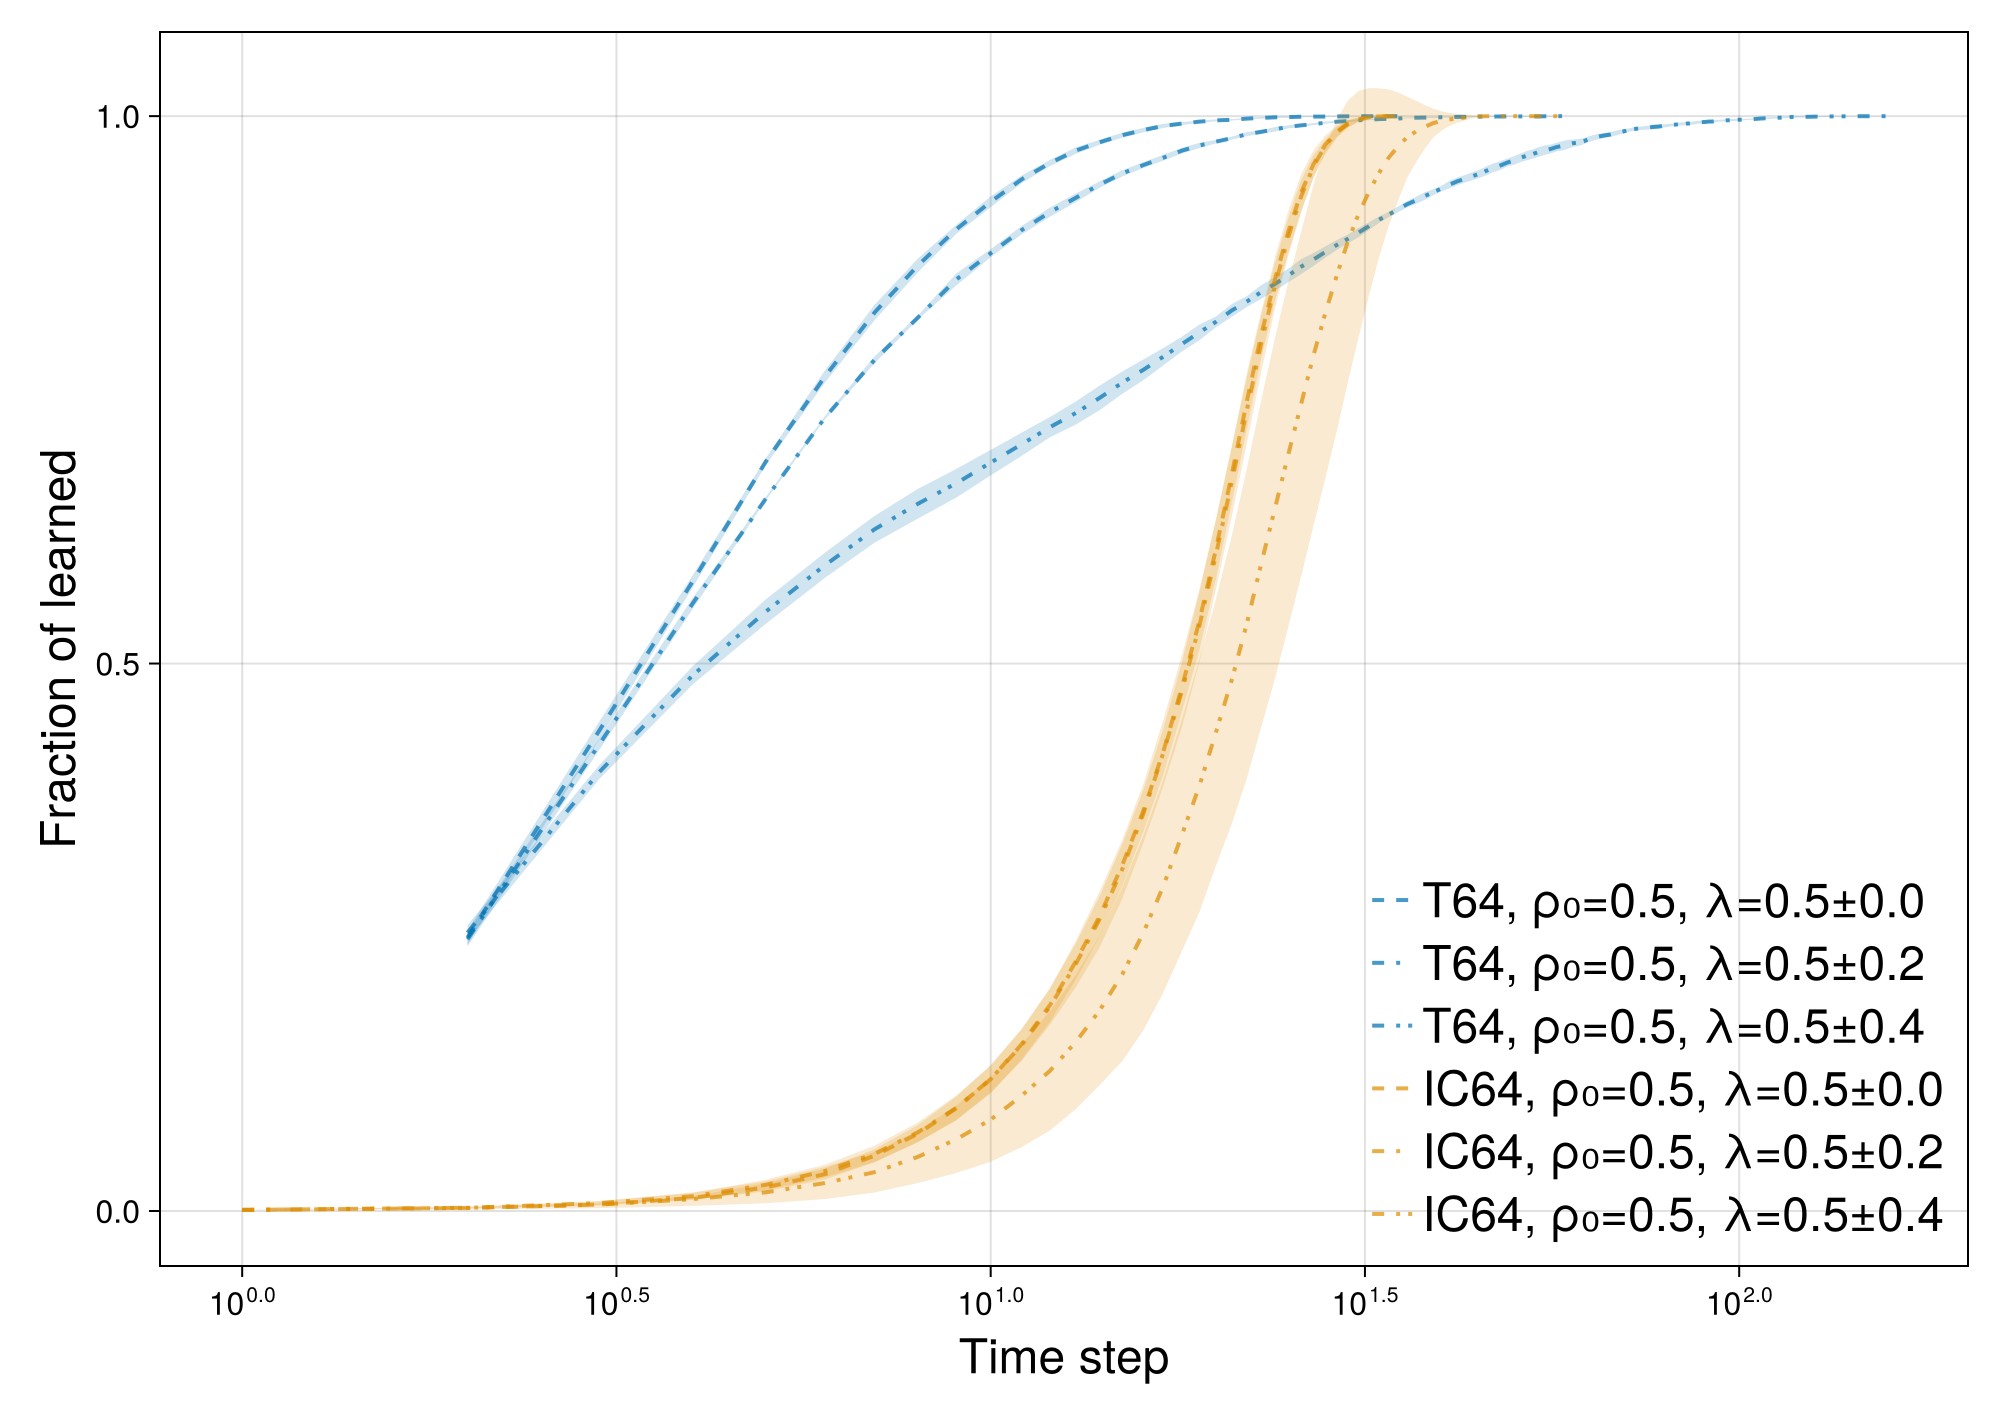
\includegraphics[width=0.45\textwidth]{figures/2D-BPCAIH-analysis/comparison plots/δλ.png}
            \caption{Comparison of learning dynamics for different learning rate heterogeneity $\delta\lambda$}
            \label{fig:comparison δλ}
        \end{figure}

        We also investigate the effects of seating arrangement for PI in Figure~\ref{fig:comparison SA}.
        For the set of parameters $\lbrace L=64,\space\rho_0=0.5,\space\delta\lambda=0.2 \rbrace$, we find that the inner corner seating arrangement performs the best in terms of both the time it takes for all the students to learn and the classroom's learning rate.
        Furthermore, we see that TI performs better than PI, especially for the earlier time steps.

        \begin{figure}[htbp!]
            \centering
            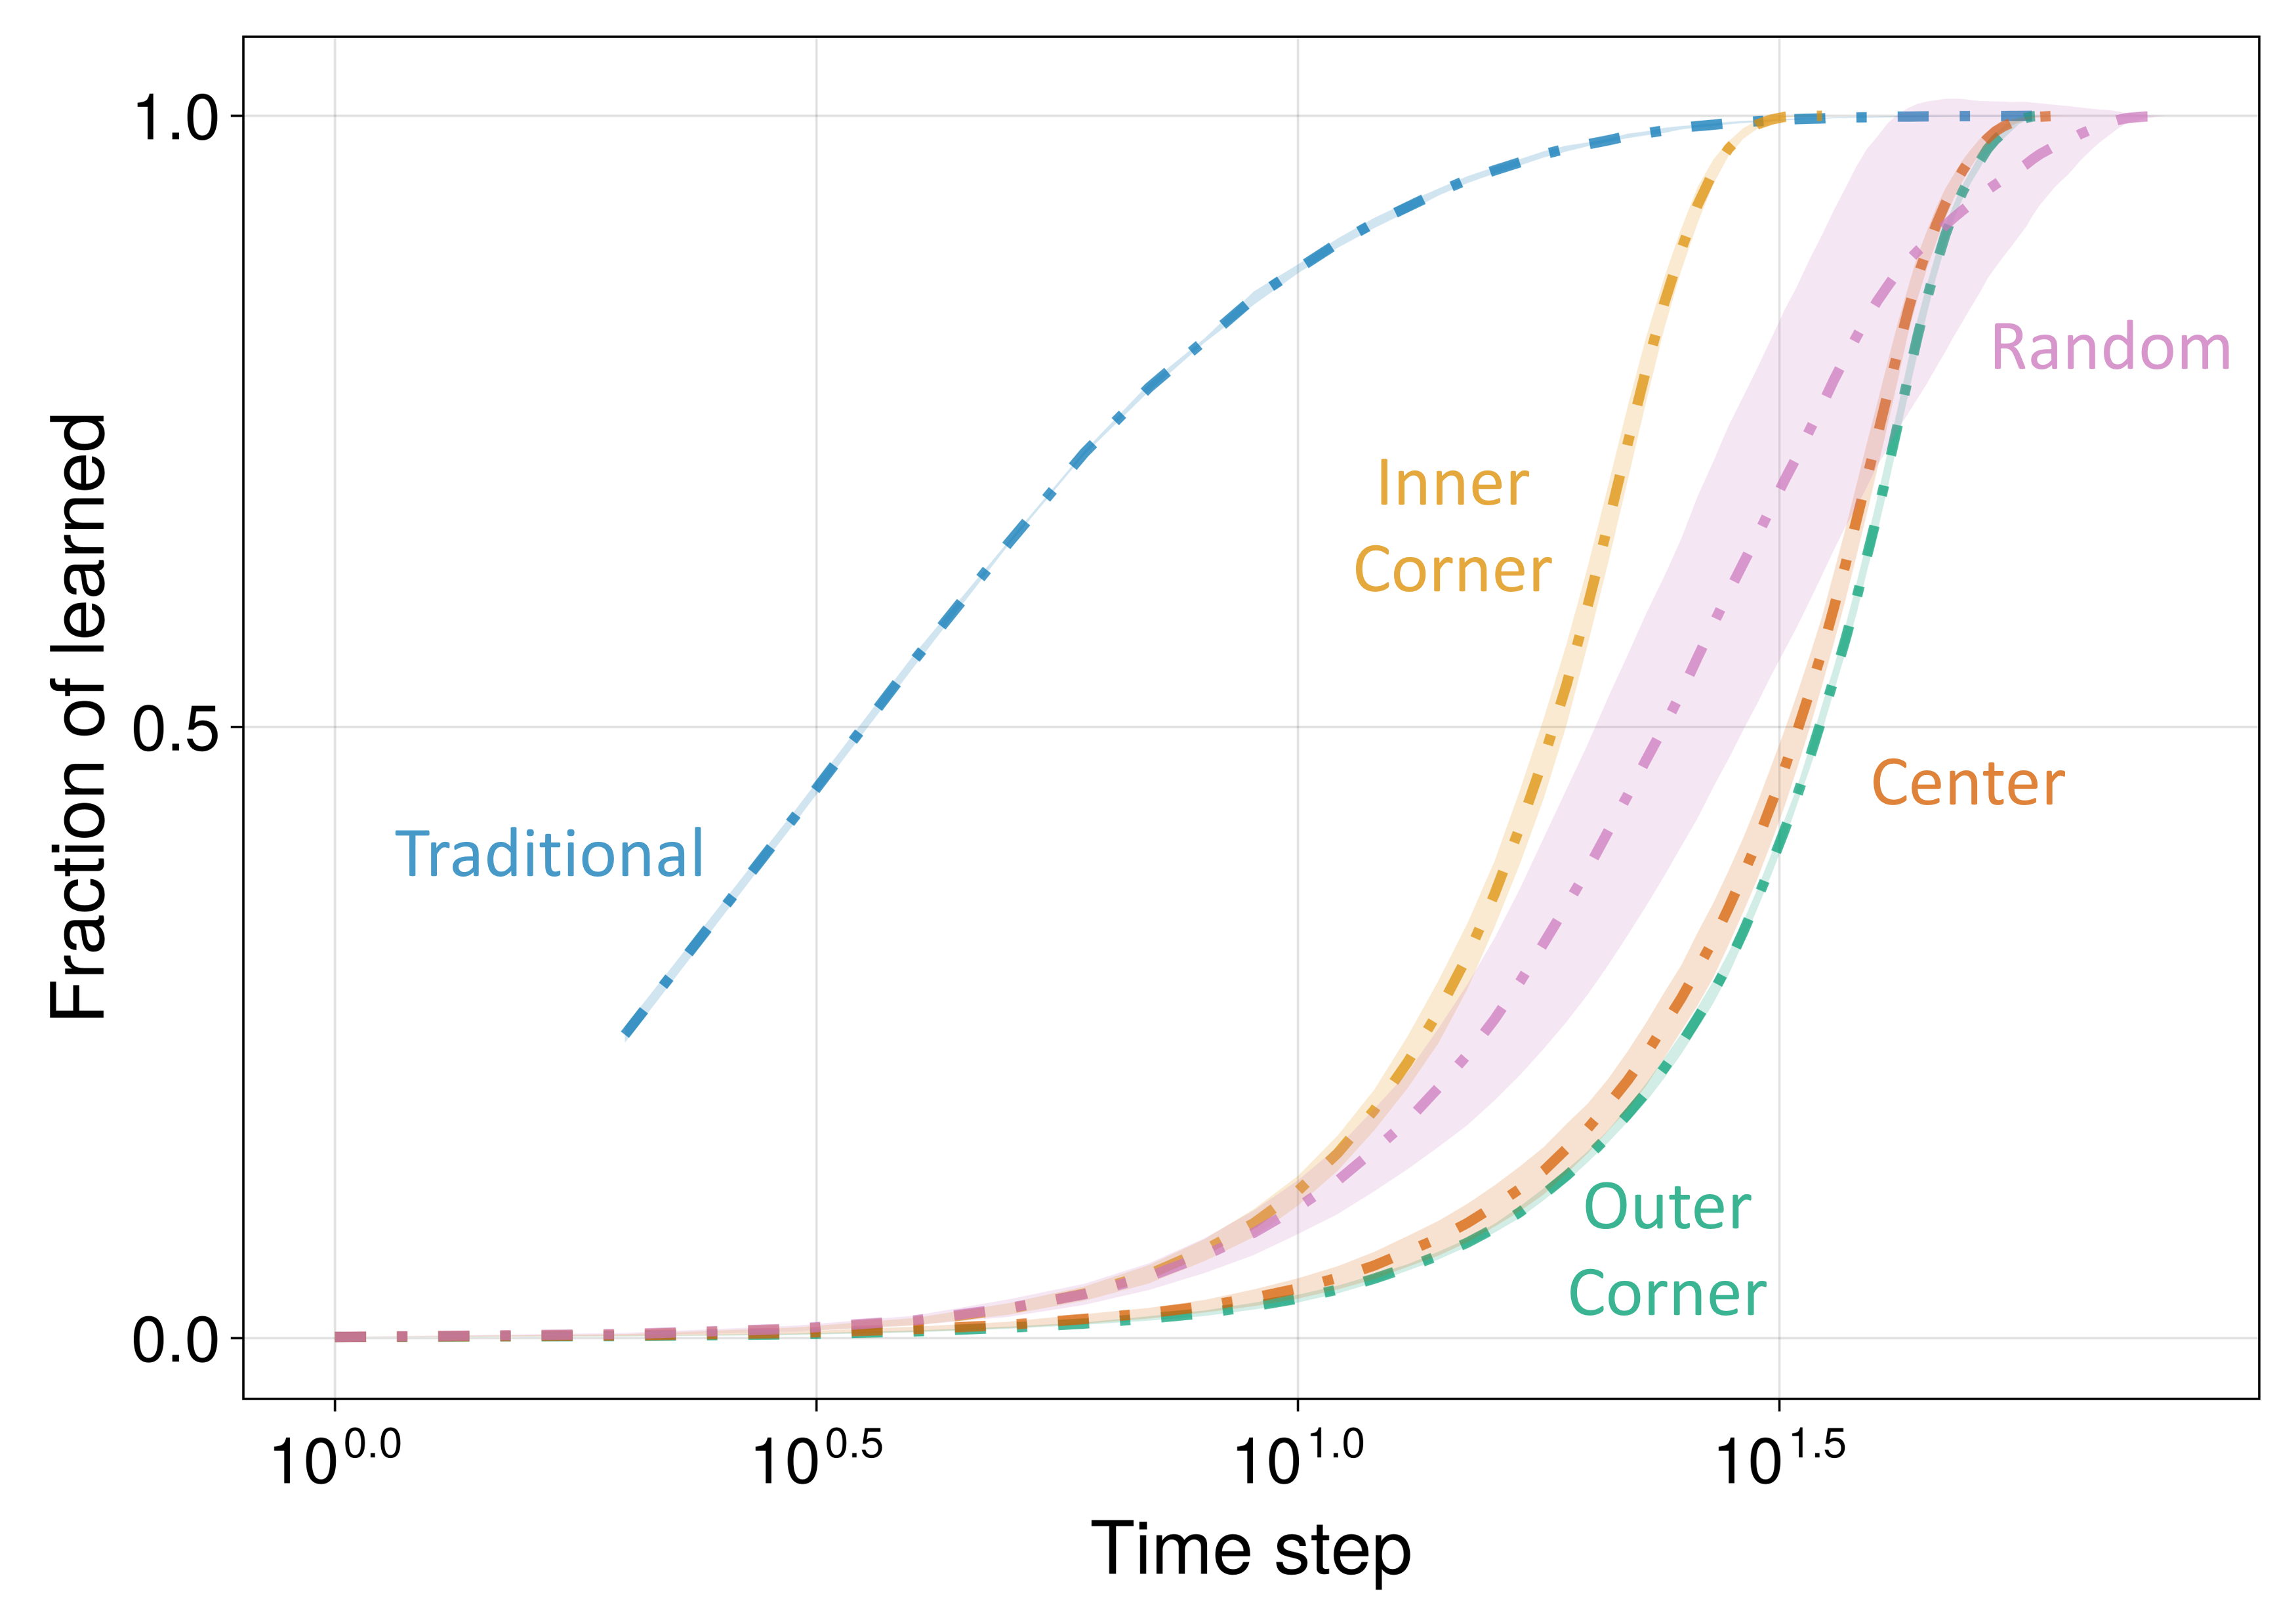
\includegraphics[width=0.45\textwidth]{figures/2D-BPCAIH-analysis/comparison plots/SA.png}
            \caption{Comparison of learning dynamics for different seating arrangements}
            \label{fig:comparison SA}
        \end{figure}

    From all the plots shown in this section, we can also observe that TI has more students learning in the earlier time steps, but has lower time to learn $t_{max}$ when compared to PI for the same set of parameters.
    This suggests that when performing TI, more time is spent waiting for slower learners than when performing PI.

    Investigating this phenomenon further, we find that the learning curve for TI has two stages: a fast initial stage and a slow final stage.
    The fast initial stage is characterized by a sharp increase in the number of learned students, this is caused by the majority of fast students learning quickly.
    The slow stage is characterized by a much slower increase in the number of learned students, this is caused by waiting for the slower students to learn.
    This phenomenon is seen in Figure~\ref{fig:comparison δλ} where the TI case where the students have a homogenous learning rate ($\delta\lambda=0$) show a consistent slope throughout the simulation compared to cases with heterogeneity ($\delta\lambda>0$) where the two-stage learning process is more evident.

    This hypothesis is further supported when investigating specific cases where the two-stage learning process is expected to be more pronounced --- classes under TI with low positional learning factor $\rho_0$ and high learning rate heterogeneity $\delta\lambda$.
    Figure~\ref{fig:two stage learning} shows one trial of a class under TI with $L=64$, $\rho_0=0.3$, and $\delta\lambda=0.4$.
    We see that for $t=2$, the majority of the student that learned are those with higher learning rates ($\lambda=0.5+0.4$).
    By $t=13$, the slower students have started to learn, but the rate of learning has slowed down significantly.
    This simulation will spend up to $t=232$ waiting for the slower students to learn.


    \begin{figure}[htbp!]
        \centering
        \subfigure[$t=2$]{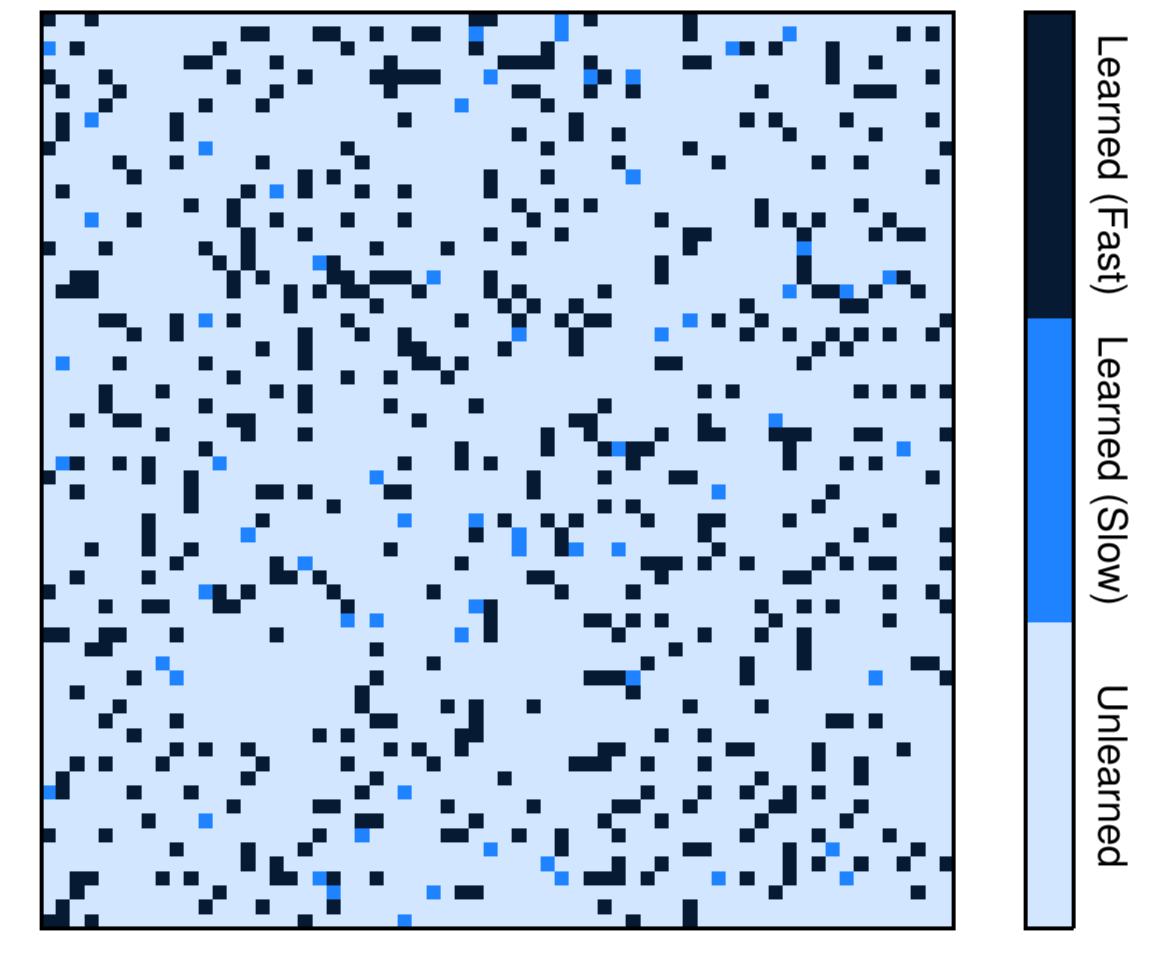
\includegraphics[width=0.23\textwidth]{figures/2D-BPCAIH-analysis/class evolutions/trad low rho high delta/2DBPCAIH-traditional-64-0.3-0.5-0.4-trial_3-2.png}}
        \subfigure[$t=13$]{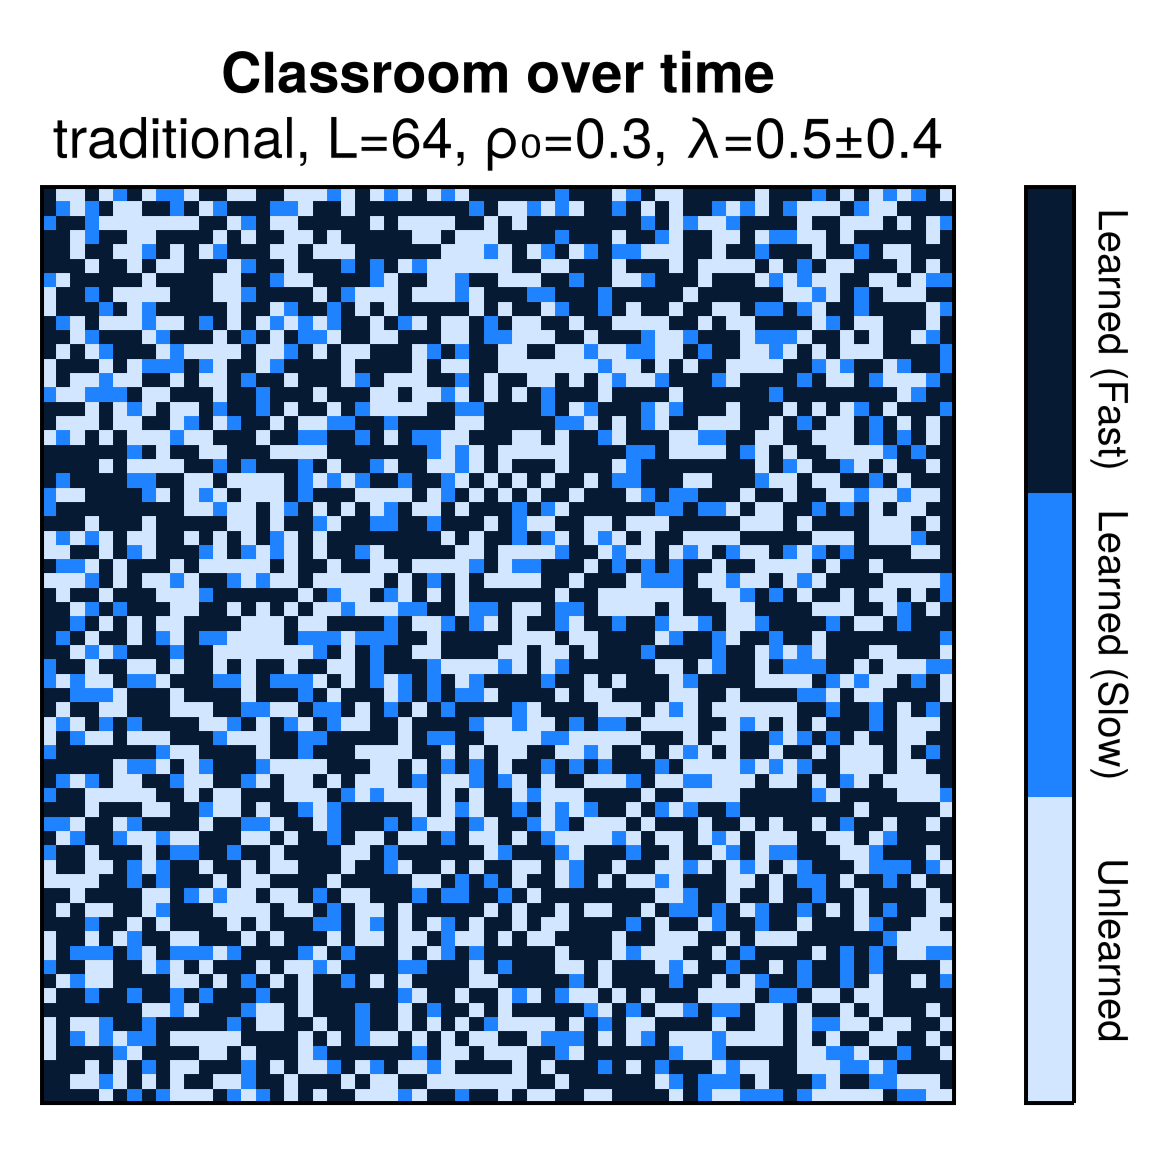
\includegraphics[width=0.23\textwidth]{figures/2D-BPCAIH-analysis/class evolutions/trad low rho high delta/2DBPCAIH-traditional-64-0.3-0.5-0.4-trial_3-13.png}}
        \caption{Two-stage learning process in traditional instruction}
        \label{fig:two stage learning}
    \end{figure}


    \subsection{Summary of effects of class size $N$, positional learning factor $\rho_0$, and learning rate heterogeneity $\delta\lambda$}

    When we compare the plot of time to learn $t_{max}$ as a function of positional learning factor $\rho_0$, and learning rate heterogeneity $\delta\lambda$ for both TI and the inner corner SA for PI, we can see that PI performs best for low values of positional learning factor $\rho_0$ and high values of learning rate heterogeneity $\delta\lambda$.
    As we vary the size of the classroom $N=L^2$, we see that breakpoints start to appear where PI performs better than TI.
    For $L=32$, PI always peforms better than TI.
    However as the classroom size increases, cases start to appear where TI performs better than PI.

    \begin{figure}[htbp!]
        \centering
        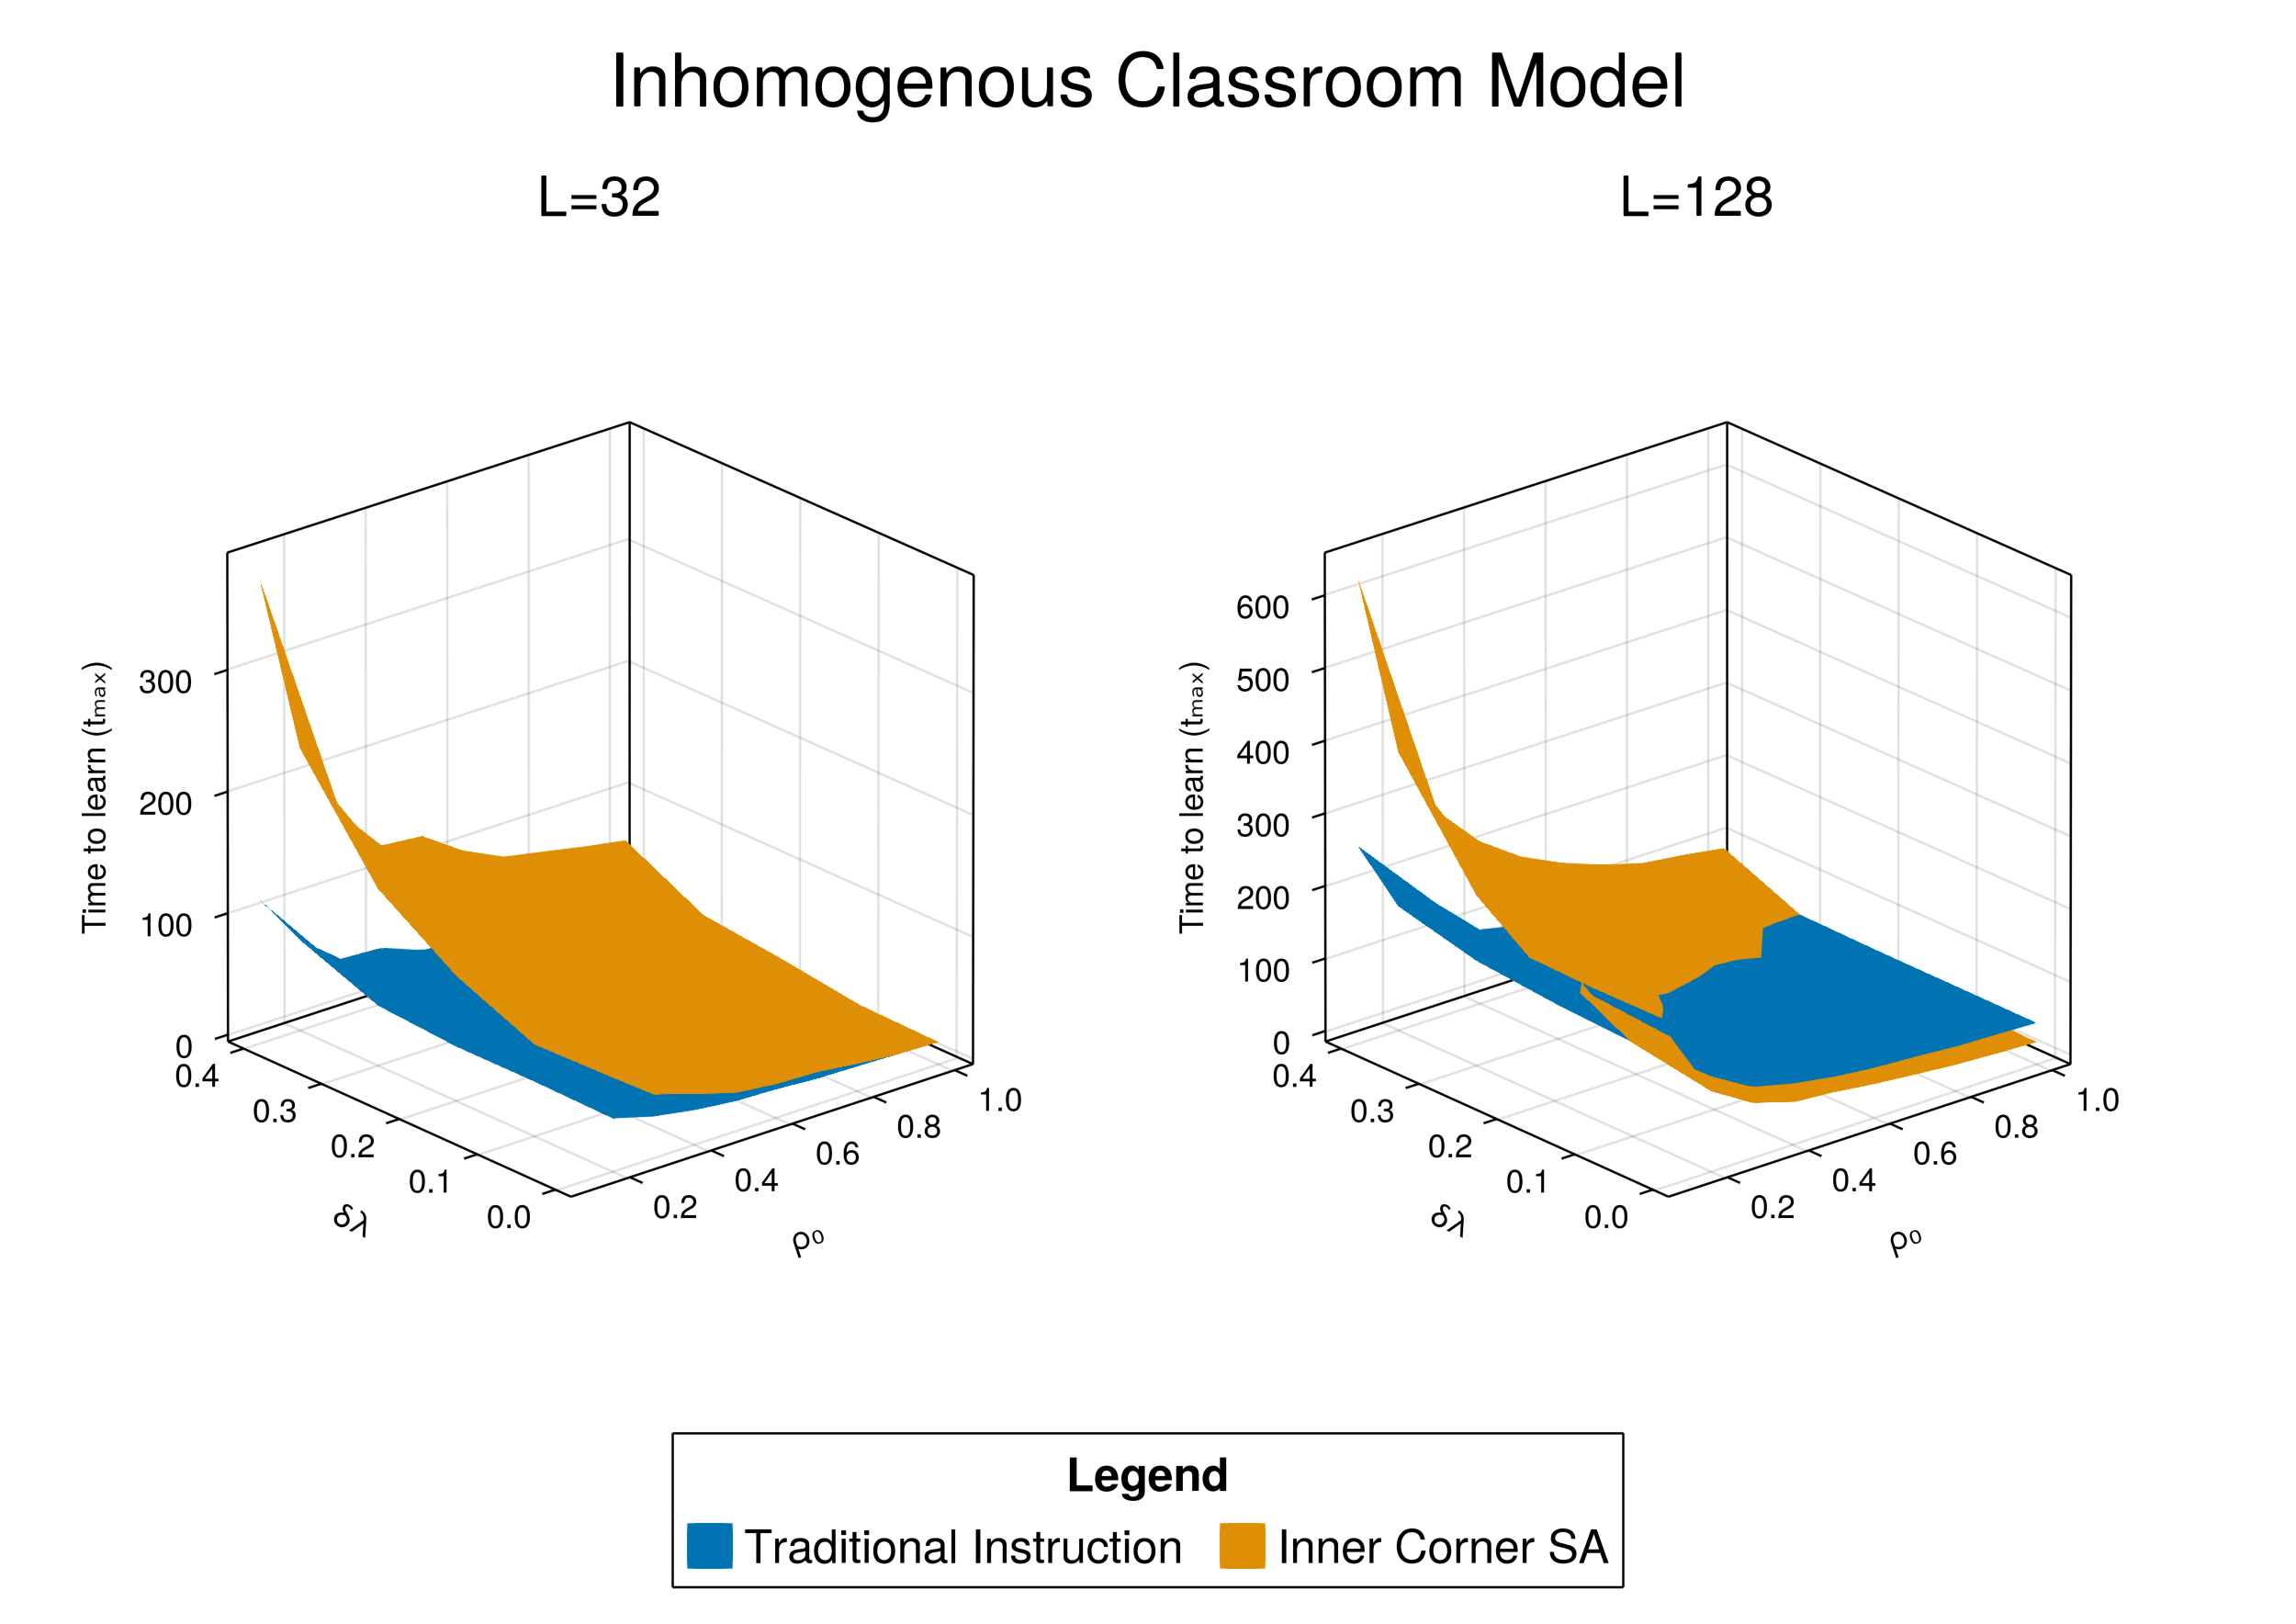
\includegraphics[width=0.47\textwidth]{figures/2D-BPCAIH-analysis/rho-dl-t plots/32-128 comparison.png}
        \caption{Summary}
        \label{fig:Params effect summary}
    \end{figure}

    
    \subsection{Return map}

    \subsection{Comparison with existing research/data}

\section{Summary and Conclusion}

\bibliography{biblio}

\end{document}

